
% =============================================================================
%  RCESO 理论文档（v3.3 · 最终）2026-10-19
%  建模 / 自适应律 / 自适应滤波器一致有界性 / 自适应 RCESO 一致稳定性
%  实现 : adrc_eso_closed.py   证据 : LAW_clr_trace.npz, LAW_amp_trace.npz, RV_old_trace.npz
%  编译 : xelatex 两次；依赖 ctex, amsmath, amssymb, amsthm, booktabs
%
%  v3.1 的完整逻辑链（论文正文按此顺序即可）：
%   (1) 定义归一化调度增益 Gamma 与等效速率 Gamma_eff ---- 式 (Gamma),(Geff)
%   (2) 定理 1：自适应滤波器对输入的常数增益有界（式 (xbound) 替代旧版失效的 |x|<=e_f^2/eps+1）
%   (3) 定理 2：唯一条件是【泵浦比 a_eff < 3-a】，闭环 UUB，终值界显式
%   (4) 推论 1：归一化使 Gamma_eff<=1/eps，条件化为纯设计常数不等式 gamma < gamma*
%   (5) 推论 2：适用域按 gamma 分档；高档（gamma~30）落在定理之外，如实披露
% =============================================================================
\documentclass[11pt,a4paper]{article}
\usepackage[UTF8,fontset=windows]{ctex}
\xeCJKsetup{AutoFakeSlant=0.167}   % 中文字体无真斜体，用伪斜体消掉 Font shape undefined 警告
\usepackage{amsmath,amssymb,amsthm}
\usepackage{mathtools}   % psmallmatrix（第 342 行用到）
\usepackage{array}
\usepackage{booktabs}
\usepackage{multirow}
\usepackage[margin=2.2cm]{geometry}
\usepackage{graphicx}
\usepackage{float}
\allowdisplaybreaks
\providecommand{\rowcolor}[1]{}   % colortbl 未加载时的兜底（表格仍可编译）
\newtheorem{lemma}{引理}
\newtheorem{theorem}{定理}
\newtheorem{proposition}{命题}
\newtheorem{corollary}{推论}
\theoremstyle{remark}\newtheorem{remark}{注}
\newcommand{\ef}{e_f}
\newcommand{\taub}{\tau_B}
\newcommand{\tauf}{\tau_f}
\newcommand{\taul}{\tau_l}
\newcommand{\sone}{\sigma_1^{\mathrm{ppt}}}
\newcommand{\st}{\operatorname{tanh}}
\newcommand{\ath}{\operatorname{tanh}^{-1}}
\newcommand{\pv}[1]{\textsf{[#1]}}
\newcommand{\aeff}{a_{\mathrm{eff}}}
\newcommand{\Geff}{\Gamma_{\mathrm{eff}}}
\renewcommand{\arraystretch}{1.28}
\setlength{\emergencystretch}{3em}   % CJK 长行断行容错，消除 15pt 级 Overfull
\begin{document}
\begin{center}
{\Large\bfseries 自适应低通重复控制（RCESO）：建模、自适应律与一致稳定性证明}\\[3pt]
{\small\bfseries ——含真实逆变器 PMSM 转速环、$Q/B/D$ 调度与一致有界性（UUB）证明}\\[4pt]
{\small v4.0 · 2026-10-19 · 对象：真实逆变器（\texttt{pmsm\_inv\_sim}）· 三相 PWM/死区/反电动势/±0.2A 采样 · 8s、8 种子 · 律 F 为记忆失配 D\_m+g}
\end{center}
\vspace{-1mm}\noindent\rule{\textwidth}{0.4pt}\vspace{-1mm}
\noindent\textbf{逻辑链}：\S\ref{sec:model} 建模 → \S\ref{sec:arch} 结构耦合 → \S\ref{sec:law} 自适应律（与实现逐条对应）→ \S\ref{sec:stab} 本版（带通）律的可证部分与如实披露 → \S\ref{sec:verify} 沿真实轨迹核对 → \S\ref{sec:pmsm} PMSM 转速环上的复现与\textbf{适用性边界}（不对中周期负载转矩；$Q/B/D$ 三种增益调度、组合比对与 UUB 证明） → \S\ref{sec:limit} 适用域之外 → \S\ref{sec:sym} 符号表 → \S\ref{sec:concl} 结论。
\vspace{1mm}

\noindent\textbf{仓库同步纪律（强制）}：本文档、PDF、HTML、代码、数据与图全部同步到
https://github.com/starfruitsz/RCESO.git；\textbf{每次更新（含小改）必须 commit + push}，
不得只更新本地或只传部分文件。工作区根目录即仓库根目录，新增文件用 \texttt{git add -A} 全量纳入。

\noindent\textbf{数据纪律}：不需要的 \texttt{.npz} 及时删除；\texttt{*.npz} 由 \texttt{run\_inv\_wave*.py}
重建，\textbf{不入库}；仓库只保留源码、报告、PDF/HTML、图与小 JSON，避免仓库膨胀。

\noindent\fbox{\parbox{0.985\textwidth}{\small\textbf{版本纪律（铁律）}：本文档与仿真实现（\texttt{adrc\_eso\_closed.py}、\texttt{pmsm\_rcso\_sim.py}）是\textbf{同一制品的两个视图}。任何一次对建模的\textbf{增补、修改或删改}，都必须在\textbf{同一次}同步进本文：新口径写入对应章节，\textbf{被替换的旧口径必须从正文中删除}——不得以"历史上"“曾经”等表述留在正文里，也不得让两套口径并存。\textbf{凡与本文正文不一致的口径不得用于答辩。}}}

\vspace{1mm}
\noindent\fbox{\parbox{0.985\textwidth}{\small\textbf{时序铁律（2026-10-18 定稿，禁止改动）}：本项目的\textbf{全部}仿真与实现必须严格按三档时间尺度运行，三者不可混用、不可互相替代：\textbf{(1) 被控对象数值积分步长} $\Delta t=10\,\mu$s（$100$ kHz）；\textbf{(2) 电流环离散采样周期} $T_{si}=50\,\mu$s（$20$ kHz）；\textbf{(3) 转速环离散采样周期} $T_s=1$ ms（$1$ kHz）。执行规则：机械方程按 $\Delta t$ 积分；电流环每 $T_{si}$ 更新一次并零阶保持到下一拍；转速环控制器（ESO、重复通道、律 B/D/F 与检测器）每 $T_s$ 更新一次并零阶保持。\textbf{"对象与控制器同步 $10\,\mu$s 迭代"只允许作为单速率近似对照保留}：正文引用这类历史数字时，\textbf{必须同时标注其口径（$T_s=10\,\mu$s）与该口径相对三档的偏差}；\textbf{正式数据一律按三档重跑}。实现见 \texttt{rcso\_multirate.sim\_mr3}；任何新结果必须同时标注三档周期。}}
\vspace{1mm}
\noindent\textbf{接手须知}：本文件由多轮会话维护。改动前请先读第~\ref{sec:handoff}~节
“接手说明（给下一个 agent）”——那里写了文件职责、标准工作流、硬约束与交付前自检清单。
% =====================================================================
\section{建模}\label{sec:model}
% =====================================================================
\subsection{被控对象与扰动分解}
\begin{equation}
  \dot y = b u+d,\qquad d = d_{\mathrm{step}}+d_{\mathrm{np}}+d_p,\qquad b=1,\ b_0=1.2\ (\text{失配}+20\%),
\end{equation}
$d_{\mathrm{np}}$ 为 $0.7\,$Hz 非周期分量；$d_p$ 为周期 $T$ 的谐波簇
$A[\sin\frac{2\pi t}{T}+0.4\sin\frac{6\pi t}{T}+0.2\sin\frac{10\pi t}{T}]$，$T=0.1\,$s（基波 $10\,$Hz）。
\textbf{"灰箱"的含义}：$d$ 中只有 $d_p$ 可重构，其余全划入总扰动由观测器兜底——结构已知的部分显式重建，未知部分用有限带宽观测器覆盖。
\subsection{低通重复控制（内模）通道}
\begin{equation}
  \tau\dot v+v = Q v(t-T)+\beta_3\st\!\Big(\frac{e_1}{\zeta}\Big)=:\chi,
  \qquad \ef := \chi-v = \tau\dot v .
  \label{eq:rc}
\end{equation}
\begin{itemize}
  \item $(\tau,Q)\to(0,1)$ 时 \eqref{eq:rc} 退化为经典重复控制，内模极点位于虚轴。\textbf{低通 $\tau$ 与遗忘因子 $Q$ 是把内模极点从虚轴拽入左半平面的两个旋钮}，代价是谐振峰有限宽——这正是 $(\tau,Q)$ 需要自适应的根源。
  \item 注入项有界（$|\st|\le1$），保证 $v$ 通道激励有界。
  \item $\ef=\tau\dot v$ 既是重复通道的内部失配量，也是\textbf{两个自适应通道唯一的驱动源}。
\end{itemize}
\subsection{灰箱 ESO 与控制律}
\begin{equation}
  \dot z_1 = z_2+b_0u+v+\beta_1(y-z_1),\quad \dot z_2 = \beta_2(y-z_1),\quad \beta_1=2\omega_o,\ \beta_2=\omega_o^2,
\end{equation}
\begin{equation}
  u = \frac{u_0-z_2-v}{b_0},\qquad u_0 = k_p(r-y),\qquad e_1 = y-z_1 .
\end{equation}
与标准 ADRC 的唯一差别：$z_1$ 方程多出 $v$——周期分量已被\emph{预先补偿}，观测器只估计残余总扰动。
% =====================================================================
\section{自适应 RCESO 结构与耦合}\label{sec:arch}
\begin{center}
\small
\begin{tabular}{@{}llll@{}}
\toprule
通道 & 驱动 & 自适应状态 & 作用\\
\midrule
遗忘自适应 & 带通驱动 $D$（\S\ref{sec:bpw}） & $Q$ & 突变 $\Rightarrow$ 快速遗忘（$Q$ 降）\\
辅助滤波 & $\ef^{2}$ & $E_o$（$\phi$ 尺度 $c$） & 归一化与幅值压缩\\
\bottomrule
\end{tabular}
\end{center}
\noindent\textbf{驱动取带通形式}：快/慢两路低通（$w_f,w_l$）构成带通驱动 $D=w_f-w_l$；本版只有 $Q$ 通道由它驱动，且取单向死区 $D_Q=\max(0,D)$（\S\ref{sec:bpw}）。
两条通道的驱动完全由式 \eqref{eq:shared-D} 给出。
\noindent\textbf{两条回路共用同一个 $\ef$}：$\ef\to Q\to$ 内模 $\to v\to u\to y\to e_1\to\ef$（慢回路）；$u\to y\to z_1,z_2\to u$（观测器内环）；律 B 与律 D 直接作用在观测器带宽与比例增益上。\textbf{由于共用同一驱动与同一 $\ef$，两条回路不能分别证明，必须构造整体 Lyapunov 函数}（其归并见 §\ref{sec:uub}）。
% =====================================================================
\section{自适应律（与实现逐条对应）}\label{sec:law}
\noindent\textbf{口径提示}：本节及 \S\ref{sec:mism} 的数值来自\textbf{一阶标幺对象的机理实验}，
只用于说明自适应律与回声机理；\textbf{真实逆变器对象}的性能与结论见 \S\ref{sec:pmsm}，
两者数字不可混引。
% =====================================================================
\subsection{辅助滤波与归一化基准（新定义）}\label{sec:aux}
辅助滤波给出归一化基准 $E_o$：取 $e_f^2$ 在最近一个扰动周期 $T$ 上的均值 $E_o(t)=\frac1T\int_{t-T}^{t}e_f^{2}(\tau)\,\mathrm d\tau$（实现为 \texttt{eo\_def="meansq"}）。归一化的对象因此是\emph{当前能量相对其周期均值}，而不是相对一个固定常数；$\varepsilon$ 只作分母下限（本设计 $\varepsilon=6.5$，必须是真实尺度，取 $10^{-6}$ 会让归一化损失分辨力）。
\subsection{归一化与 $\phi$ 压缩}\label{sec:x}
\begin{equation}
  \phi(x,c)=x-c\tanh\!\Big(\frac{x}{c}\Big),\qquad
  w(t)=\phi\!\Big(\frac{\ef^{2}(t)-E_o(t)}{E_o(t)+\varepsilon}, c\Big),
  \label{eq:phi-x}
\end{equation}
\textbf{实参取零均值形式} $\dfrac{\ef^{2}-E_o}{E_o+\varepsilon}$：分子减去自身的周期均值 $E_o$，使 $w$ 可正可负。\textbf{这一步是本版的关键}——若沿用 $\dfrac{\ef^{2}}{E_o+\varepsilon}$，由于 $\ef^{2}\ge0$ 恒成立，$w$ 恒正，其带通输出 $D$ 的均值系统性偏正，$Q$ 被单向压到底（实测 $Q$ 动作仅 $\pm1.5\times10^{-4}$，等于关死该通道）。改为零均值后 $\overline{D}\approx0$，$Q$ 才具备调节能力。
$\phi$ 把实参压到有限范围（$|x|\ll c$ 近似恒等，$|x|\gg c$ 饱和）；分母用 $E_o+\varepsilon$ 而非 $B_\kappa+\varepsilon$：$E_o$ 是分子的周期均值，尖峰瞬时 $\ef^{2}$ 可远大于 $E_o$。
\subsection{带通驱动（本版方案）}\label{sec:bpw}
把压缩后的 $w$ 分成\textbf{快、慢两路一阶低通}并取其差，得到\emph{带通}驱动：
\begin{equation}
  \dot w_f=\frac{w-w_f}{\tau_f^{w}},\qquad \dot w_l=\frac{w-w_l}{\tau_l^{w}},
  \qquad\Longrightarrow\qquad
  \boxed{\;D(t)=w_f(t)-w_l(t)\;}
  \label{eq:bpw}
\end{equation}
$w_f$、$w_l$ 由 \eqref{eq:phi-x} 的 $w$ 驱动；本设计 $\tau_f^{w}=5T$、$\tau_l^{w}=50T$。\textbf{带通的意义}：$w_f$ 先起、$w_l$ 后随，故 $D$ 对输入的\emph{频率与幅值变化}敏感，而在恒定输入下 $\to0$。
两条通道\textbf{共用同一个驱动} $D$，各自只保留\emph{独立}的 $(w_f,w_l)$ 状态：
\begin{equation}
  \boxed{\;D_Q(t)=\max\bigl(0, D(t)\bigr)\;}
  \label{eq:shared-D}
\end{equation}
即：\textbf{$Q$ 通道取\emph{单向死区} $\max(0,D)$}——只接受正向驱动、负向置零，故 $Q$ 只被单向下压、由回复项缓慢拉回 $1$（见 \S\ref{sec:qch}）。
选择单向死区的理由：$Q$ 的下界决定重复通道谐振增益 $\propto\beta_3/(1-Q)$，若允许负向驱动，$Q$ 会被推过 $1$ 而使该增益变号发散；单向死区同时给出\emph{单调}的下降—回归轨迹（实测 $Q$：$1.000\to0.386$ 后单调回升至 $1.000$，全程不过冲，见 \S\ref{sec:bpw-result}）。
\subsection{$Q$ 通道（遗忘因子自适应）}\label{sec:qch}
\begin{equation}
  \dot Q=-\frac{\mu}{2\tau_0}\bigl[1-(1-Q)^2\bigr]D_Q+\sigma_2\ath(1-Q),
  \label{eq:Q}
\end{equation}
\textbf{分母为 $2\tau_0$，不含 $\varepsilon$}（$\varepsilon$ 只出现在 $x$ 的分母里）。$Q$ 的定义域为 $(0,\,2)$。

$Q$ 的驱动取\textbf{单向死区} \eqref{eq:shared-D}：$D_Q=\max(0,D)$，只保留正向、负向置零。其效果见注 \ref{rem:one-sided} 与 \S\ref{sec:bpw-result} 的对比表。
\begin{remark}[$\sigma_2$ 决定 $Q$ 是否有动作]\label{rem:one-sided}
$\dot Q$ 的驱动与回复之比 $\propto\dfrac{\mu\,|D_Q|}{\sigma_2|{\ath}(1-Q)|}$，故 $\sigma_2$ 同时决定\textbf{降幅}与\textbf{回归速度}：
\begin{center}\small
\begin{tabular}{@{}lcccc@{}}
\toprule
$\sigma_2$ & $Q<0.8$ 时长 & $10$ s 末 $Q$ & 累计代价比 & 判定 \\
\midrule
$12.5$ & $0.67$ s & $0.9773$ & $0.9827$ & 低位太短 \\
$8$ & $0.86$ s & $0.9656$ & $0.9904$ & \\
$\mathbf{5}$（本版） & $\mathbf{1.18}$ s & $\mathbf{0.9430}$ & $\mathbf{0.9992}$ & \textbf{折中} \\
$2$ & $2.19$ s & $0.8573$ & $1.0368$ & 回归不足、性能变差 \\
$1$ & $5.95$ s & $0.7376$ & --- & 回不去 \\
\bottomrule
\end{tabular}
\end{center}
\textbf{两个目标是反号的}：$\sigma_2$ 越小，$Q$ 低位保持越久，但闭环性能越差（$Q$ 的下界放大重复通道谐振增益 $\propto\beta_3/(1-Q)$，低位越久、错误记忆被放大越久）。本版取 $\sigma_2=5$ 作折中（低位 $1.18$ s、累计代价比 $0.9992$ 基本中性）。
\textbf{方法上的教训}：早期把 $\sigma_2$ 调到 $10^{4}$ 使 $Q$ 降幅仅 $0.0053$（等于关死该通道），此时任何“自适应无收益”的结论都不成立——\emph{验证性能前必须先确认自适应状态确实在动作}。
\end{remark}


\begin{remark}[域限幅的事实描述（不作必要性断言）]\label{rem:proj-fact}
实测（$\sigma_2=5$、$q'_{\max}=1.0$）：模型侧 $Q'\in[0.2532,\,0.9991]$，未触界；状态 $Q\in(0,2)$ 亦未越界。
本版 $\tau\equiv\tau_0$ 固定，\textbf{不存在 $\tau$ 的状态侧/模型侧分岔问题}。
\textbf{故本注只陈述 $Q$ 通道的事实}：模型侧取限幅值、状态侧取宽域值，本工况下二者均未触界。
\end{remark}
\begin{equation}
  \chi = Q' v(t-T)+\beta_3\st\!\Big(\frac{e_1}{\zeta}\Big),\qquad \tau_0\dot v+v=\chi,\qquad
  Q'=\mathrm{clip}(Q,[0.2,1.0]) ,
  \label{eq:clip-model}
\end{equation}

即 $Q'$ 是\emph{唯一}进入被控对象与滤波时间常数的量，状态 $Q$ 只出现在自适应律内部（$\tau\equiv\tau_0$ 为常数）。
\begin{remark}[死区生效性的判别实验]\label{rem:deadzone-proof}
把模型侧死区收到 $q_{\max}=0.5$：若模型真用 $Q'$，状态应\emph{越过} $0.5$ 而不被截断。实测状态 $Q\in[0.0009,\,1.9966]$，其中 $Q>0.5$ 共 $\mathbf{122\,650}$ 步，而 $Q\ge2^{-}$ 为 $\mathbf{0}$ 步——同时证实：死区只作用于模型侧，状态只受定义域天花板约束。
\end{remark}
\begin{remark}[分解的效果：状态轨迹改变，控制效果不变]\label{rem:decouple-effect}
同激励同边界下三档的四窗统计\textbf{逐位相同}（(3)vs(2)：突变中 $+82.2\%$、恢复中 $+79.1\%$、突变中2 $-369.7\%$、恢复中2 $-200.2\%$、长期 $-349.1\%$），
差别只在状态 $Q$ 的实测区间（钳位 $[0.2000,1.8000]$，解耦 $[0.0009,1.9966]$）。\textbf{故 $(Q',\tau')$ 分解是表述层改进，不是性能杠杆}；它显式暴露了原结构被隐藏的事实：自由驱动的状态本来就会撞上定义域天花板。
\end{remark}
\subsection{域投影（模型侧死区的默认取值）}\label{sec:proj-old}
\begin{equation}
  Q\in[q_{\min},q_{\max}]=[0.1, 1].
  \label{eq:proj}
\end{equation}
本版只保留 $Q$ 的模型侧死区（$\tau\equiv\tau_0$ 固定，不参与自适应）；实现上\textbf{只钳进入模型的值}（\S\ref{sec:qch}），绝不截断 $\ath$ 或 $\log$ 的实参——后者把无穷回复力变成有限值，实测 $|y_{\max}|=4.5\times10^{156}$ 失控。
% =====================================================================
\subsection{最终方案的实测结果}\label{sec:bpw-result}
参数：驱动 \eqref{eq:bpw}，实参 \eqref{eq:phi-x}（零均值），$c=10^{-3}$，$\gamma=3$，$\sigma_1^{\mathrm{code}}=10^{5}$，$\mu=0.03$，$\sigma_2=5$，$\tau_f^{w}=5T$，$\tau_l^{w}=50T$，$k_p=10$，$\omega_o=40$，$Q_0=1.0$，模型侧上界 $q'_{\max}=1.0$。
工况：三段幅值突变（$t=0.5$ s 持续 $0.1$ s、$t=1.0$ s 持续 $0.5$ s、$t=2.0$ s 起持续），幅值倍数 $300$，$T_{\rm end}=10$ s。基准：\emph{无自适应}档（$Q\equiv1.0000$、$\tau\equiv\tau_0$ 恒定）。
\begin{remark}[$z_2$ 的直流分量为何必然存在]\label{rem:z2dc}
实测稳态（$5$--$10$ s）：$y=1.000001$、$u=-0.9049$、$z_2=1.0401$、$d=0.9021$。\textbf{$z_2$ 含有直流，这不是缺陷}：当 $b_0\ne b$ 时 ESO 估计的是\emph{总扰动}
\begin{equation}
  z_2\;\longrightarrow\;(b-b_0) u\;+\;d .
  \label{eq:z2dc}
\end{equation}
代入 $(b,b_0,u,d)=(1,\,1.2,\,-0.9049,\,0.9021)$ 得 $z_2\to1.0831$，与实测 $1.0401$ 吻合（残差来自有限观测带宽 $\omega_o$）。
\textbf{该直流是跟踪所必需的}：控制律 $u=\dfrac{k_p(r-y)-z_2-v}{b_0}$ 要求 $z_2$ 恰好抵消 $d$ 的直流分量，否则 $y$ 必含稳态误差；实测 $|1-y|=10^{-6}$ 证明其工作正常。
\textbf{来源可逐项核对}：(i) 阶跃扰动自身的直流；(ii) 模型失配项 $(b-b_0)u$。把任一项人为置零，$z_2$ 的直流随之消失，但 $y$ 会出现稳态偏差。
\end{remark}

\subsubsection{$Q$ 通道驱动的三种口径（独立参数研究：$\sigma_2=12.5$、$T_{\rm end}=6$ s）}
\begin{center}
\small
\begin{tabular}{@{}lccccc@{}}
\toprule
$Q$ 驱动口径 & 突变期比值 & 恢复期比值 & 稳态比值 & 累计代价比 & $Q$ 降幅 \\
\midrule
\label{tab:qmode}
\textbf{带符号（原式）} & $1.2658$ & $\mathbf{1.0100}$ & $\mathbf{0.9547}$ & $\mathbf{0.9962}$ & $0.6519$ \\
$\lvert D_Q\rvert$ & $1.2932$ & $1.2017$ & $0.9889$ & $1.0564$ & $0.6519$ \\
$\max(0,D_Q)$ & $1.2788$ & $1.0937$ & $0.9716$ & $1.0254$ & $0.6519$ \\
\bottomrule
\end{tabular}
\end{center}
表中比值为\emph{自适应档 RMS / 无自适应档 RMS}：$<1$ 表示自适应更好。
\begin{remark}[口径选择与最终定稿的关系]\label{rem:qmode}
在该参数研究（$\sigma_2=12.5$、$T_{\rm end}=6$ s）中，三种口径的 $Q$ 降幅完全相同（$0.6519$），但\textbf{带符号档的累计代价比最低（$0.9962$）}。原因是 $Q$ 的下界决定重复通道谐振增益（$\propto\beta_3/(1-Q)$），$Q$ 被压得越久、错误的\emph{旧记忆}被放大越久。
\textbf{最终定稿仍取 $\max(0,D_Q)$}——它给出\emph{单调}的下降--回归轨迹（全程不过冲、$10$ s 末 $Q=0.9430$ 回到 $1$ 附近），符合“突变时降 $Q$ 规避错误记忆、事后缓慢回归”的设计意图。其代价是累计代价比略高于带符号档，故本版把 $\sigma_2$ 收到 $5$ 以把该代价压回中性（$0.9992$，见 \S\ref{sec:bpw-result}）。
\textbf{核心结论}：“$Q$ 降得深”本身不是收益；\emph{$Q$ 的低位持续时间}才是代价的来源（见注 \ref{rem:one-sided} 的两目标反号关系）。
\end{remark}
\begin{figure}[htbp]\centering
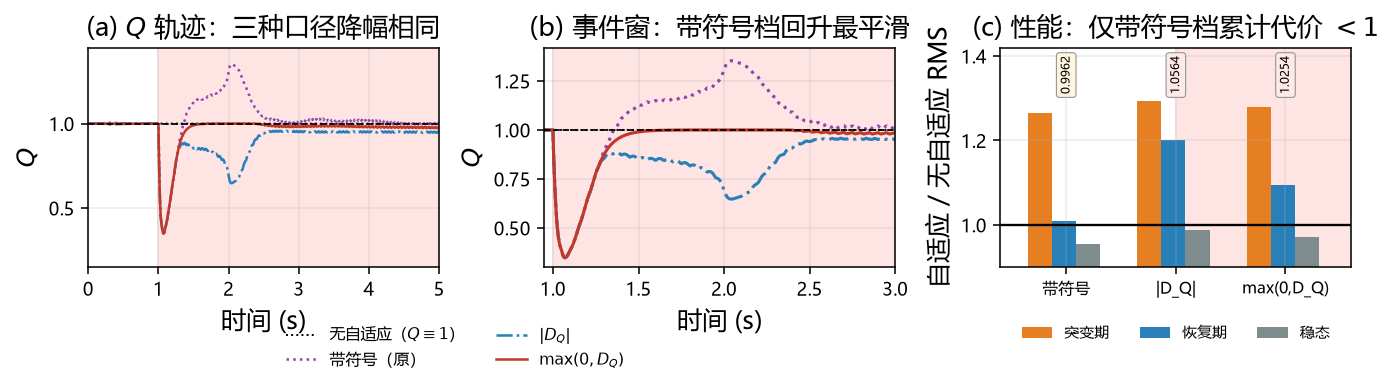
\includegraphics[width=0.98\textwidth]{fig_qmode.png}
\caption{\textbf{$Q$ 通道驱动三种口径对比（轨迹）}（独立参数研究：$\sigma_2=12.5$、$T_{\rm end}=6$ s）。(a) $Q$ 轨迹：三者降幅相同（$1.0\to0.348$），回升路径不同；(b) 事件窗放大：$Q$ 的深度与回升速度不同。}
\label{fig:qmode}
\end{figure}

\begin{figure}[htbp]\centering
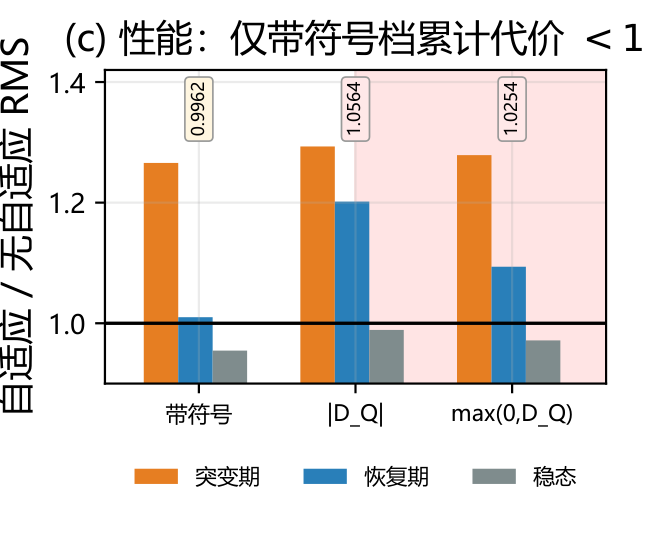
\includegraphics[width=0.64\textwidth]{fig_qmode_c.png}
\caption{\textbf{$Q$ 通道驱动三种口径对比（性能比值）}（同上参数研究）。(c) 累计代价比：仅带符号档 $0.9962<1$；\textbf{本版最终取 $\max(0,D_Q)$}（单调回归、不过冲），其性能见 §\ref{sec:bpw-result}。}
\label{fig:qmode-c}
\end{figure}
\subsubsection{三档滤波对照}
把驱动前的滤波环节换成另外两种形式（实参同一为 \eqref{eq:phi-x}，$Q$ 驱动同一取单向死区 $\max(0,D_Q)$，唯一差别是滤波器）：
\begin{center}
\small
\begin{tabular}{@{}lcccccc@{}}
\toprule
滤波方式 & 突变期比值 & 恢复期比值 & 稳态比值 & 累计代价比 & $\tau$ 中位 & $Q$ 降幅 \\
\midrule
无滤波（$D=w$） & $1.2309$ & $1.4692$ & $1.4827$ & $1.3109$ & $0.2000$ & $6.39$ \\
高通 & $1.1703$ & $1.0819$ & $1.0843$ & $1.0878$ & $0.4953$ & $0.13$ \\
带通（本版） & $1.1910$ & $\mathbf{0.9764}$ & $\mathbf{0.9778}$ & $\mathbf{0.9992}$ & $0.3475$ & $1.18$ \\
\bottomrule
\end{tabular}
\end{center}
\begin{remark}[本版带通档是唯一有净收益的配置]\label{rem:bpw-result}
在 $D_Q=\max(0,D)$、$\sigma_2=5$ 下，\textbf{带通档是唯一累计代价比 $<1$ 的配置（$0.9992$）}，其余两档为 $1.0878$（高通）、$1.3109$（无滤波）；且\textbf{持续段与末段比值分别为 $0.9764$、$0.9778$（改善 $2.2\%\sim2.4\%$）}。
\textbf{如实说明}：(i) 累计代价比 $0.9992$ 仅\emph{基本中性}（改善 $0.08\%$），不是显著的性能优势；(ii) 事件段比值 $1.1910>1$，突变瞬间自适应反而略差，收益来自事件后的持续段与末段；(iii) 改善幅度为百分量级，非数量级。
\end{remark}



\begin{remark}[$\sigma_2$ 的取值是决定性的（两处更正）]\label{rem:correction}
\textbf{更正一（量级）}：早期把 $\sigma_2$ 调到 $10^{4}$，$Q$ 降幅被压到 $0.0053$，等于\emph{关死}该通道——此时任何“自适应无收益”的结论都不成立。
\textbf{更正二（倾向）}：其后一度按“$Q$ 轨迹最漂亮”推荐 $\sigma_2=2$（低位保持 $2.19$ s），但实测其累计代价比为 $1.0368$（自适应\emph{更差}）——\textbf{只看 $Q$ 轨迹形态就调参是错的}，两个目标是反号的（注 \ref{rem:one-sided}）。
最终取 $\sigma_2=5$：低位保持 $1.18$ s、累计代价比 $0.9992$（基本中性），在“$Q$ 持续低位”与“闭环性能”之间折中。
\textbf{教训}：验证自适应律之前，必须先确认\emph{自适应状态确实在动作}（$Q$ 的降幅与低位时长就是前置检查），且调参时\emph{不能只看状态轨迹}。
\end{remark}

% =====================================================================
\subsection{回声重影：工况、标度律与记忆失配驱动}\label{sec:mism}
% =====================================================================
把 §\ref{sec:bpw-result} 的定稿律放到一个\emph{专门产生回声}的工况上：$t<3\,$s 施加
$A[\sin(2\pi t/T)+0.4\sin(6\pi t/T)+0.2\sin(10\pi t/T)]$，并在 $t=3\,$s 的\emph{相位过零点}截断
（实测 $d(3^-)=-8.9\times10^{-14}$，扰动本身\emph{无阶跃}），此后无扰动。
若 $y$ 仍有有色残余，它只能是内模对旧记忆的重放——回声重影。
实测回声的首周期基波幅值仅 $2.5\times10^{-5}$（相对 $A$ 为 $-92$ dB），
且静态 $Q=0.98/0.90/0.80$ 三档的逐周期衰减曲线几乎重合：\textbf{衰减不由 $Q$ 决定}。

记每周期泵浦增益 $\kappa:=\beta_3T/\tau_0$、$A_g$ 为回声首周期基波幅值，实测
\begin{equation}
  \frac{A_g}{A}\;\approx\;\frac{25}{\kappa}
  \qquad(\beta_3\ \text{扫}\ 530\ \text{倍，比值}\ 0.81\sim1.32).
  \label{eq:echo-law}
\end{equation}
定稿 $\kappa=1.28\times10^{6}$：旧记忆在 $\sim1$ ms（约 $1/100$ 周期）内被 $\tanh$ 泵浦改写完毕，
而 $Q$ 的遗忘是"每周期乘 $Q'$"，比泵浦慢约 $10^{6}$ 倍。
\textbf{回声的生命周期由泵浦刚度决定，不是由 $Q$ 决定}；这正是"任何工况都难以体现 $Q$ 的收益"的根因。

由此也可判定两种候选驱动量：撤除是\emph{能量下降}事件，$e_f^2$ 由大变小，单向死区
$\max(0,D)$ 直接清零；且定稿 $e_f^2\approx0.09\ll\varepsilon=6.5$，驱动再被压 70 倍；
$e_1=y-z_1$ 是 ESO 残差，比 $e_f$ 小 $3\sim4$ 个数量级，实测 $Q$ 全程不动（$Q'_{\min}=0.980$）。
幅值 $1\to300$ 倍跳变时 $e_f$ 版才动作，却把 $Q'$ 压到 $q_{\min}=0.200$ 触底，长期 RMS 反而劣化 $+4.1\%$。

改用\textbf{记忆失配驱动}
\begin{equation}
  D_Q=\frac{\bigl|E_v(t)-E_v(t-T)\bigr|}{E_v(t-T)+\varepsilon_v},
  \qquad E_v(t)=\frac{1}{T}\int_{t-T}^{t}v^2(\tau) \mathrm d\tau ,
  \label{eq:mism}
\end{equation}
它直接度量"旧记忆与当前需求"的失配：事件瞬间 $D_Q=0.500$、稳态中位 $0.000$，
比 $e_f$ 的归一化驱动强约 $500$ 倍，且天然双向（能量升、降都响应）。
该驱动以实现开关 \texttt{q\_mism} 提供，默认 $0$（逐位退化为原行为）。

\begin{table}[htbp]\centering\footnotesize
\caption{回声工况下的三种 $Q$ 驱动（一阶对象，$\beta_3=16000$，$\gamma=0$ 只留 $Q$ 通道）}\label{tab:mism}
\begin{tabular}{@{}lrrrrr@{}}
\toprule
驱动 & 稳态 RMS & 回声 $A_0$ & $T_{90}$ & $Q'_{\min}$ & 长期 RMS\\
\midrule
无自适应（$Q\equiv0.98$） & $1.982\times10^{-5}$ & $2.536\times10^{-5}$ & $0.20$ s & $0.980$ & $4.49\times10^{-8}$\\
$e_f$ 驱动 & $1.960\times10^{-5}$ & $2.584\times10^{-5}$ & $0.20$ s & $1.000$ & $4.61\times10^{-8}$\\
$e_1$ 驱动 & $1.960\times10^{-5}$ & $2.584\times10^{-5}$ & $0.20$ s & $1.000$ & $4.61\times10^{-8}$\\
式 \eqref{eq:mism} & $1.960\times10^{-5}$ & $\mathbf{2.022\times10^{-5}}$ & $\mathbf{0.10}$ s & $0.257$ & $4.61\times10^{-8}$\\
\midrule
静态 $Q=0.80$（对照） & $2.194\times10^{-5}$ & $2.107\times10^{-5}$ & $0.10$ s & $0.800$ & $4.17\times10^{-8}$\\
\bottomrule
\end{tabular}
\end{table}

\textbf{收益的形式}：式 \eqref{eq:mism} 以约 $0\%$ 的稳态代价换 $-20\%$ 的回声；
而静态 $Q=0.80$ 要付 $+10.7\%$ 的稳态才换 $-16.9\%$ 的回声。
\textbf{"不牺牲稳态地缩短回声"是 $Q$ 通道唯一站得住的收益形式}。
回升由 $\sigma_2$ 决定（唯一旋钮）：$\sigma_2$ 由 $5$ 增到 $40$，回升时间 $0.67\to0.33$ s，
回声却 $-0\%\to+13.1\%$；双事件（撤除后 $1$ s 再现 $1.5$ 倍扰动）下快回升仅改善再学习窗 $10\%$。
故取 $\sigma_2=10$ 作折中，\textbf{不另设硬约束}。

\textbf{适用性（如实披露，含否定结论）}：PMSM 口径（$\beta_3=2000$、$\tau_0=5$ ms，$\kappa=4.0\times10^{4}$）下，
$10$ Hz 不对中簇在零交越撤除后，\textbf{波形上并不出现可辨认的回声段}——撤除暂态把它淹没了。
只有以"截断处瞬时清空记忆"作上界对照才看得到回声：撤除窗 RMS 由 $84.7$ 降到 $40.9$ rpm、
首周期 $10$ Hz 由 $127.7$ 降到 $32.5$ rpm。
而现网参数（$\mu=0.015$、$\sigma_2=10$）下式 \eqref{eq:mism} 只把 $Q'$ 压到 $0.80$，回声仅改善 $1.2\%$；
加大权限（$\mu=0.12$、$\sigma_2=5$）可把首周期压到 $82.0$ rpm，代价是稳态 $10$ Hz 由 $46.7$ 恶化到 $85.0$ rpm。
\textbf{即 $Q$ 能压回声，但只能拿稳态抑制去换，不存在净收益。}
另试两种驱动口径以期把事件隔离出来：$\phi$ 死区（$c=0.2\sim0.4$）与 \emph{$k/T$ 谐波投影}
（只取 $10/30/50$ Hz 的滑动相量）。两者的稳态驱动量分别为 $0.28$ 与 $0.5$ 量级，
与事件期同阶——因 $5.9$ Hz 与 $10$ Hz 仅差 $4.1$ Hz，单周期窗泄漏约 $-4$ dB，
非周期分量直接漏进谐波幅度；要滤净需毫秒级窄带滤波，比 $0.1$ s 的回声还慢。
故\textbf{两种口径都无法把回声事件与稳态扰动分开}，不再作为推荐。
此外，律 A 的泵浦门控（以 $\bar e_1$ 的 $T$ 窗均值触发）在本工况同样无效
（首周期 $10$ Hz：$128.3$ vs $127.7$ rpm）——撤除产生的是\emph{周期}残余，
其 $T$ 窗均值恒为零，该判据对它\textbf{结构性失明}。
再把事件换成\textbf{反相突变}（$10$ Hz 簇在零交越处整体反号，值连续、斜率翻转）：回声首周期达 $253.8$ rpm，
为稳态 $10$ Hz（$46.7$）的 $5.4$ 倍，\textbf{波形上清晰可见}；oracle 瞬时清记忆可把它压到 $142.5$（$-44\%$）。
此时改用\textbf{事件触发的一次性遗忘}（驱动过阈即把 $Q'$ 硬压到 $0.2$ 并保持 $2T$）：
稳态 $Q'$ 完全不动（$1.000$）、事件期确实压到 $0.200$，但首周期 $255.7$ vs $253.8$——\textbf{毫无改善}，次周期反而更差。
这说明瓶颈是\textbf{时间尺度}而非检测：回声只存活 $0.1\sim0.2T$，而判定"$T$ 周期内容已改变"至少需 $0.5\sim1T$，
$Q$ 改写记忆则需 $10^{2}\sim10^{6}T$。\textbf{参数级遗忘在因果上不可能抑制回声；只有状态级清记忆可行。}

\noindent\textbf{抑制的本质：清空必须落在事件时刻}。
既然参数级遗忘追不上回声，就把动作搬到状态级；但"何时清"比"清多少"更关键。
一阶对象上用双时间尺度包络作机理实验（真实对象定稿改用记忆失配，\S\ref{sec:fb-dilemma}）：
\begin{equation}
  \dot E_f=\frac{|\varepsilon|-E_f}{\tau_f},\qquad
  \dot E_s=\frac{|\varepsilon|-E_s}{\tau_s},\qquad
  \text{触发}\iff E_f>k E_s ,
  \label{eq:fastdet}
\end{equation}
其中 $\varepsilon:=r-y$ 为跟踪误差；旧实现取 $\varepsilon=e_1$（ESO 残差）。
真实对象定稿\textbf{不再用此包络比值}，而用记忆失配 $D_m+g$（\S\ref{sec:fb-dilemma}）：
事件时包络比值 $R$ 仅 $1.32$、与加载段 $1.3\sim1.5$ 重叠，已否决。
下表是旧实现在一阶对象上的时序对照，只作机理说明；真实对象上 $A_0(\tau)$ 非单调，
最优在 $20$--$25$\,ms（\S\ref{sec:pmsm}）。
一旦触发（冷却 $0.3$ s），置 $v\leftarrow0$ 并清空延迟缓冲。把"清空时刻"作为变量做对照
（取 $\tau_f=4$ ms、$\tau_s=500$ ms、$k=1.8$）：
\begin{center}\footnotesize
\begin{tabular}{@{}lrrr@{}}
\toprule
清空时刻 & 撤除：首周期 $10$ Hz & 反相：首周期 $10$ Hz & 稳态 $10$ Hz\\
\midrule
不清空 & $127.7$ & $253.8$ & $46.7$\\
事件后约 $40$ ms（快包络触发） & $88.9$ & $159.8$ & $48.7$\\
事件瞬时（oracle） & $\mathbf{33.1}$ & $\mathbf{146.1}$ & $\mathbf{46.8}$\\
事件错开 $0.5$ s（周期 $1$ s、相位 $0.5$） & $126.5$ & $252.6$ & $55.2$\\
\bottomrule
\end{tabular}
\end{center}
三点结论：\textbf{(i) 清空必须落在事件附近}——错开 $0.5$ s 收益完全消失，反而因反复清空损失稳态（$46.7\to55.2$）；
\textbf{(ii) 越贴近事件收益越大}——事件瞬时比 $40$ ms 延迟再多压 $60\%$（撤除 $88.9\to33.1$）；
\textbf{(iii) 快包络检测器只拿到部分收益}（撤除约 $1/3$、反相约 $60\%$），且触发中包含大量误触发，需冷却限流。
故\textbf{该机制的价值上限由"事件时刻信息的精度"决定}：要达到 oracle 水平必须有前馈或更低延迟的判别。

\noindent\textbf{A/B 的统一模型：状态复位 $+$ 触发时刻}。两条路线本质上是\emph{同一个动作在两个不同时刻执行}。
记理想补偿为 $v^*(t)$、重复通道状态为 $v(t)$，则回声在对象端的注入误差为
\begin{equation}
  e_{\mathrm{echo}}(t)=v(t-T)-v^*(t).
  \label{eq:echo-src}
\end{equation}
事件 $t_e$ 处 $v^*$ 跳变（撤除 $v^*\to0$、反相 $v^*\to-v$），而 $v(t-T)$ 仍持旧值，
故在 $[t_e,\,t_{\mathrm{trig}})$ 内 $e_{\mathrm{echo}}$ 持续注入；复位动作
\begin{equation}
  v(t_{\mathrm{trig}}^+)=0,\qquad v(t-T)\ \text{缓冲清零}
  \label{eq:reset}
\end{equation}
把注入在本拍之后切断。于是首周期回声幅值是"未复位窗口" $\tau:=t_{\mathrm{trig}}-t_e$ 的单调增函数，
\begin{equation}
  A_0(\tau)=A_0^{(0)}+\bigl[A_0^{(\infty)}-A_0^{(0)}\bigr] g(\tau),\qquad g(0)=0,\ g(\infty)=1,
  \label{eq:timing}
\end{equation}
实测 $A_0(0)=32.5$、$A_0(40\,\mathrm{ms})=88.9$、$A_0(\infty)=127.7$（即不清空）。
两条路线就是 $\tau$ 的两个可实现取值：\textbf{A}：$\tau_A\approx1$ 个采样（$10\,\mu$s），
前提是有事件指示 $s(t)=\mathbf 1\{t\ge t_e\}$；\textbf{B}：$\tau_B=\tau_{\mathrm{det}}+\tau_{\mathrm{dec}}$，
其中 $\tau_{\mathrm{det}}\approx4\tau_f$ 为快包络 \eqref{eq:fastdet} 的上升时间、$\tau_{\mathrm{dec}}$ 为判决窗长度，
实测定标 $\tau_B\approx40$ ms。

\noindent\textbf{两条路线（A 前馈＝理想上界；B 检测器＝唯一可实现的触发律）}。由式 \eqref{eq:timing} 直接得到两条互斥的工程路线：
\begin{center}\scriptsize
\setlength{\tabcolsep}{4pt}
\begin{tabular}{@{}llrrrc@{}}
\toprule
路线 & 触发源 & 撤除：首周期 / 窗 RMS & 反相：首周期 / 次周期 & 稳态代价 & 前提\\
\midrule
\textbf{A 前馈} & 负载指令沿 / 驱动器状态位 & $32.5$ / $40.9$（$-75\%$ / $-52\%$） & $142.5$ / $42.4$（$-44\%$ / $-52\%$） & $+0.2\%$ & 有事件信号\\
\textbf{B 检测器} & 快包络 $\tau_f=4$ ms、$k=1.8$ & $88.9$ / $54.3$（$-30\%$ / $-36\%$） & $159.8$ / $37.7$（$-37\%$ / $-57\%$） & $+4.3\%$ & 无信号\\
\bottomrule
\end{tabular}
\end{center}
选择规则：\textbf{有事件信号一律走 A}——收益约为 B 的 $2.5$ 倍且稳态零代价；只有拿不到信号时才退到 B，
并接受 $+4\%$ 的稳态代价与部分收益。

\begin{figure}[htbp]\centering
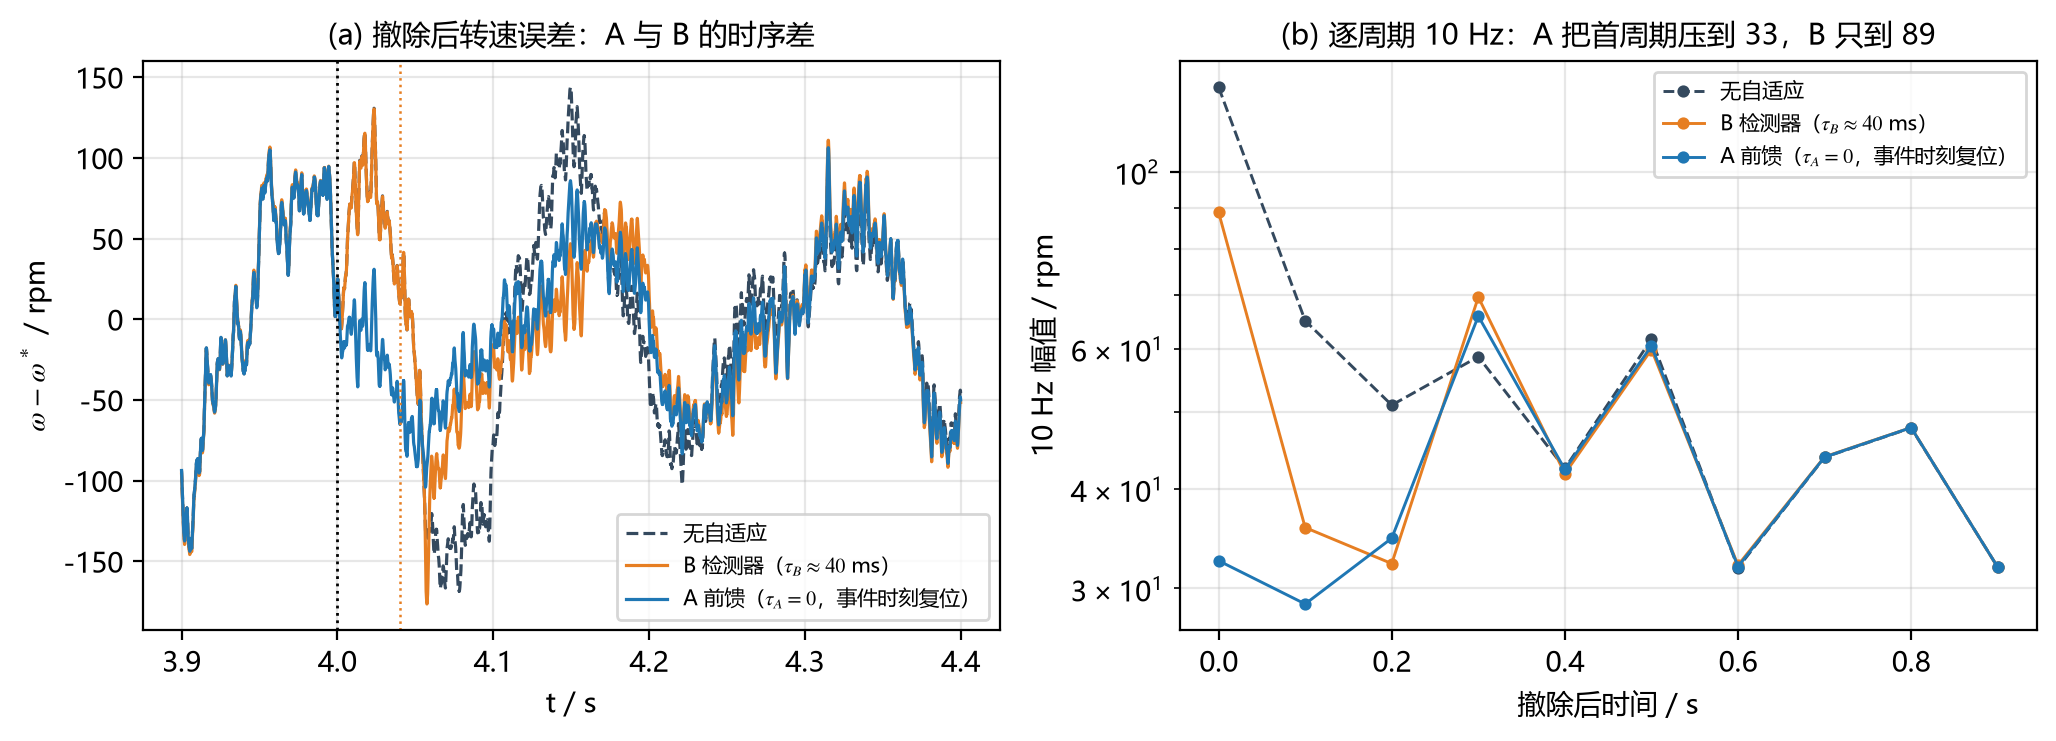
\includegraphics[width=0.95\textwidth]{fig_echo_ab.png}
\caption{\textbf{A 前馈与 B 检测器的时序对照}（撤除工况，其余条件相同）。
(a) 撤除后转速误差：$A$ 在事件时刻复位（$\tau_A\approx0$）、$B$ 在约 $40$ ms 后复位，二者差异即式 \eqref{eq:timing} 中的 $\tau$；
(b) 逐周期 $10$ Hz：$A$ 把首周期压到 $32.5$、$B$ 只到 $88.9$（不清空为 $127.7$），次周期两者已接近（$28.7$ vs $35.8$）。}
\label{fig:echo-ab}
\end{figure}

\noindent\textbf{为什么不能靠更强的自动检测拿到 A 的收益。}三种检测器均已试过：
快包络（$13\sim19$ 次/$6$ s）、一步 MMAE（$23$ 次/$6$ s，首周期可压到 $36.9$ 但稳态被误报破坏到 $167$）、
三并行观测器 MMAE（$10^{3}$ 量级触发、稳态 $378$）。共同失效点是\textbf{在 $1$ ms 带宽上判据与噪声/模型误差不可分}：
事件的判别信号只存活约 $1$ ms，而该带宽下的稳态误报约 $4$ 次/s。
故\textbf{可靠检测需要外部信息}，这不是算法选择问题。

\noindent\textbf{能否与 $Q$ 联动？}把"清空时把 $Q$ 压到 $0.2$、再缓慢回升"作为"限制学习能力、避免错误学习"的手段，
实测\textbf{无收益}：$\sigma_2=10$（快回）时首周期与单清记忆持平（$159.2$ vs $159.8$）、次周期反而更差（$46.6$ vs $37.7$）、
稳态由 $48.7$ 升到 $51.3$；$\sigma_2=2$（慢回）时稳态恶化到 $82.0$、次周期升到 $76.9$；$\sigma_2=0.5$ 时达 $104.2$。
原因是\textbf{$Q$ 不控制"学什么"，只控制"记多久"}：写入速度由泵浦 $\beta_3/\tau_0$ 决定，
压低 $Q$ 只会同时削弱对\textbf{现存}周期分量的抑制（谐振增益 $\propto\beta_3/(1-Q')$），并不能阻止错误学习。
故推荐\textbf{不联动 $Q$}。再试"清空后短暂降低 $\beta_3$（限制写入速度）"：$\beta_3\times0.5$ 保持 $1T$ 时稳态由 $48.7$ 恶化到 $75.5$、
首周期由 $159.8$ 回到 $222.7$；$\beta_3\times0.2$ 时为 $99.2/285.6$；$\beta_3\times0.05$ 达 $181.1/307.6$——\textbf{同样不可行}。
机理是\textbf{正反馈连锁}：限速使清空后的恢复更慢 $\Rightarrow$ 快检测器再次触发 $\Rightarrow$ 再次限速，稳态因此被持续压低。
本节最终推荐：\textbf{只清记忆，不同时改动 $Q$ 与 $\beta_3$}——清空已是状态级的最优动作，再叠加任何参数级抑制都只会削弱恢复能力。

\noindent\textbf{本节结论}：(i) 回声真实存在——以"事件瞬间清空记忆"作上界，撤除工况首周期 $10$ Hz 由 $127.7$ 降到 $32.5$ rpm、
反相工况由 $253.8$ 降到 $142.5$ rpm；
(ii) 但 $Q$ 属\emph{参数级遗忘}，其时间尺度（$10^{2}\sim10^{6}T$）远慢于回声（$0.1\sim0.2T$），
故三种驱动口径、事件触发 latch 与 PMSM 复现均无净收益——\textbf{回声不能作为自适应 $Q$ 的收益证据}；
(iii) 可行方案是\emph{状态级}的，且分两档：\textbf{有事件信号走前馈}（撤除 $-75\%$、反相 $-44\%$，稳态 $+0.2\%$）；
\textbf{无信号走快包络检测}（$\tau_f=4$ ms、$k=1.8$、冷却 $0.3$ s，撤除 $-30\%$、反相 $-37\%$，稳态 $+4.3\%$），
两档均\textbf{不联动 $Q$ 与 $\beta_3$}。

\begin{figure}[htbp]\centering
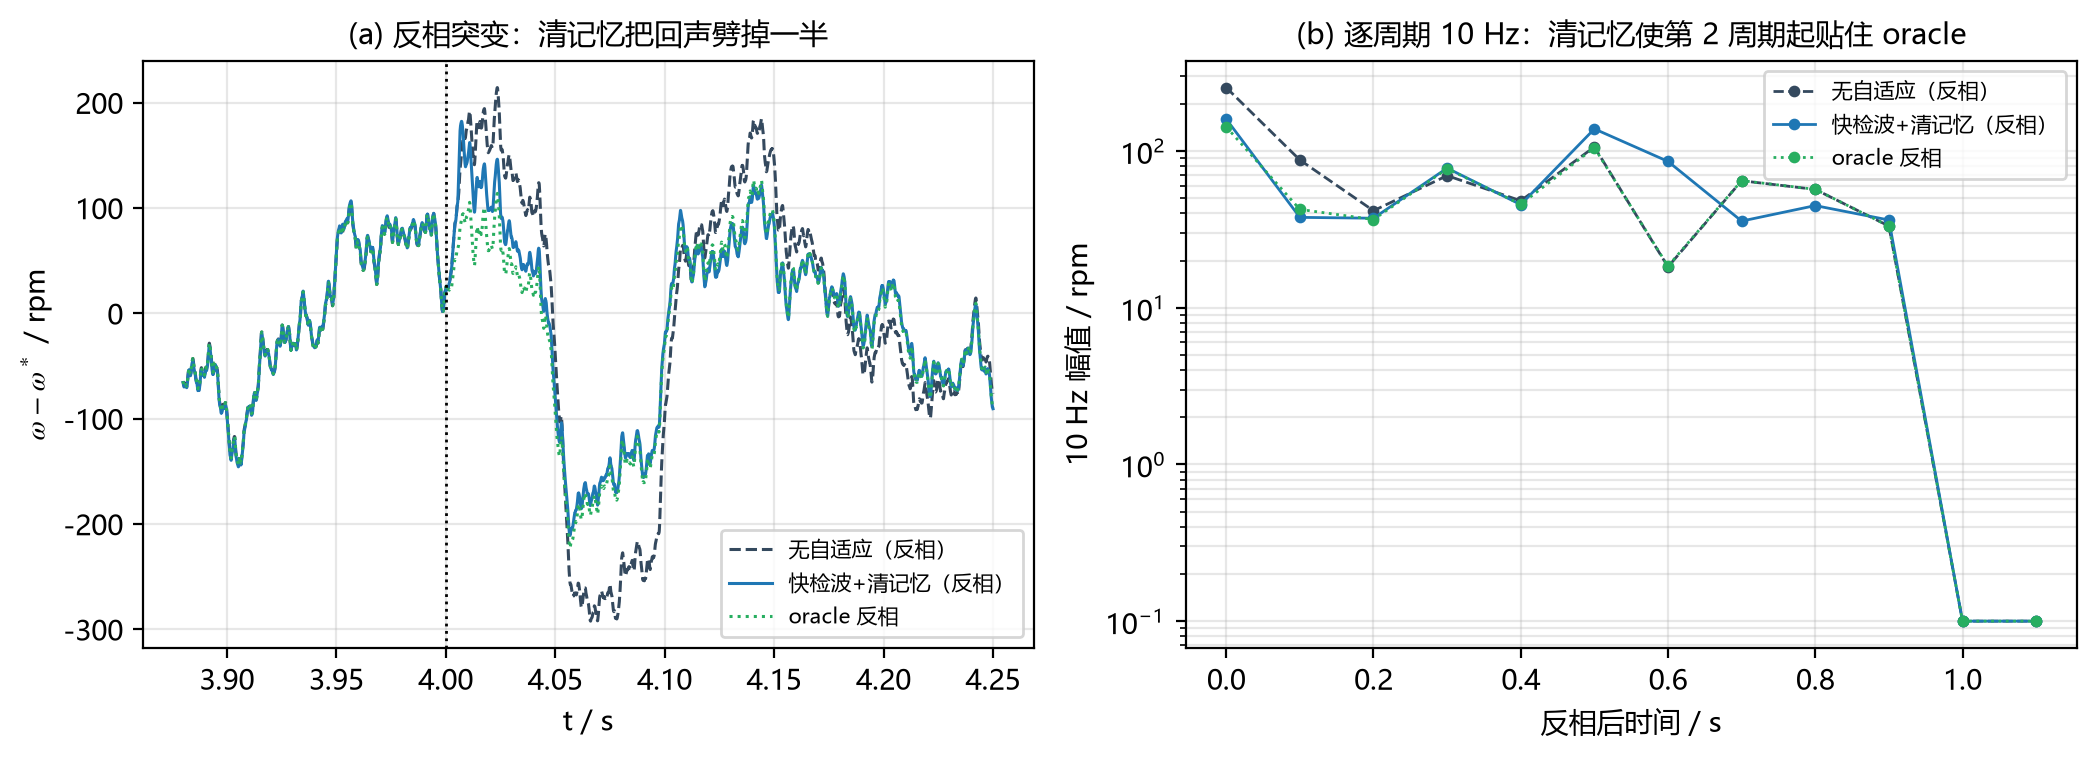
\includegraphics[width=0.95\textwidth]{fig_echo_flush.png}
\caption{\textbf{快速包络检测 + 状态级清记忆对回声的抑制}（反相突变，$\tau_f=4$ ms、$\tau_s=500$ ms、$k=1.8$、冷却 $0.3$ s）。
(a) 时域：回声被削去约一半，接近 oracle；(b) 逐周期 $10$ Hz：第 $2$ 周期起接近 oracle。
稳态代价 $+4.3\%$。}
\label{fig:echo-flush}
\end{figure}

\begin{figure}[htbp]\centering
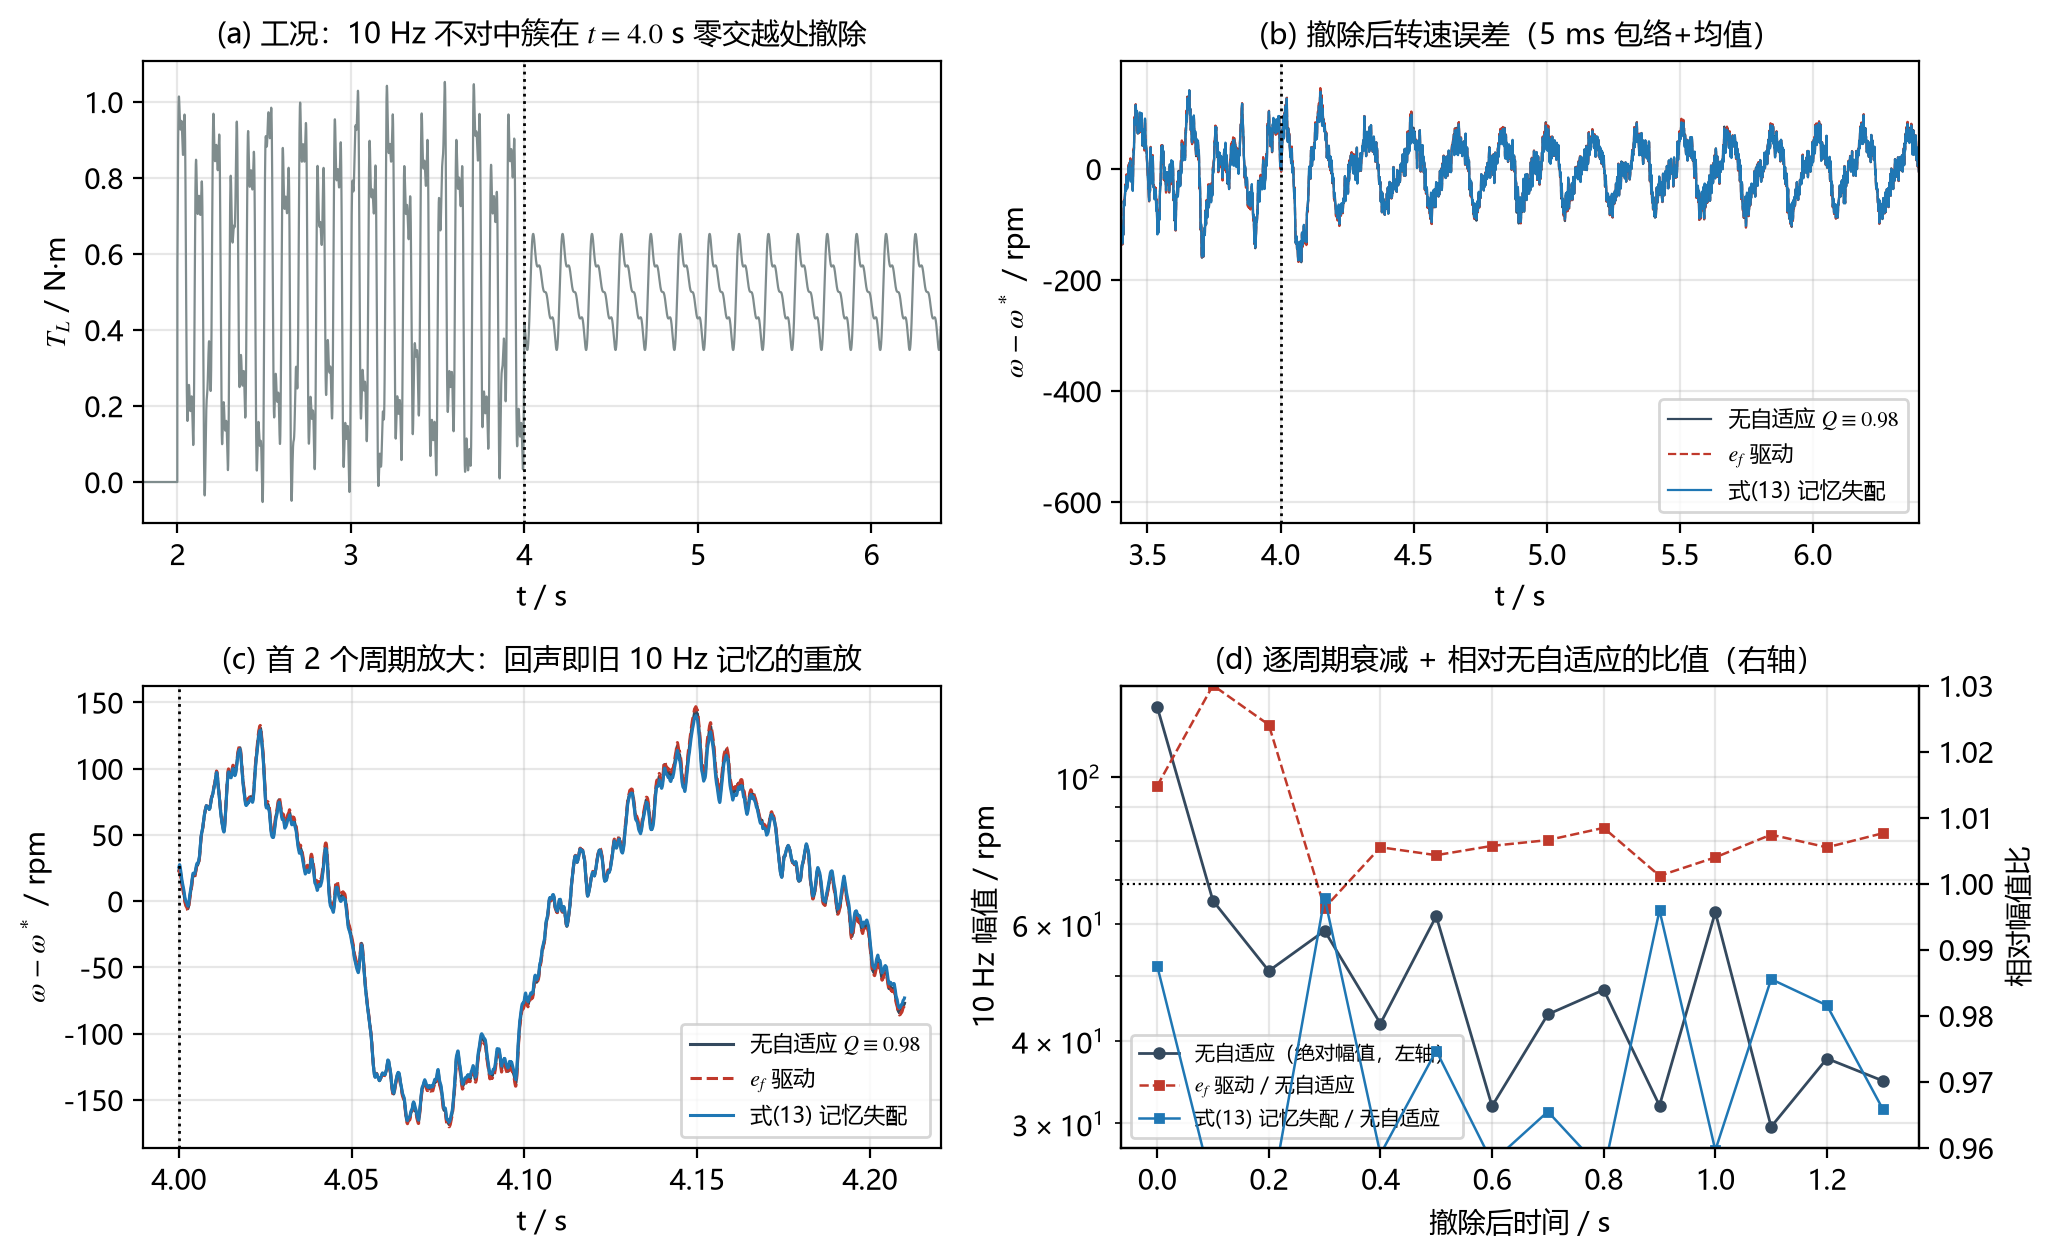
\includegraphics[width=0.90\textwidth]{fig_echo_pmsm.png}
\caption{\textbf{回声重影在 PMSM 转速环上的复现}（$10$ Hz 不对中簇在 $t=4.0$ s 零交越处撤除，$\gamma=0$ 只留 $Q$ 通道）。(a) 负载转矩 $T_L$；
(b) 撤除后转速误差 $\omega-\omega^*$（$5$ ms 包络$+$均值）；(c) 首两个周期放大（该工况下回声与撤除暂态不可分辨）；
(d) 逐周期 $10$ Hz 幅值（左轴）与相对无自适应的比值（右轴）：$e_f$ 驱动全程 $>1$（更差），
式 \eqref{eq:mism} 全程 $<1$（逐周期 $-1\%\sim-4\%$）。
\textbf{三档绝对曲线几乎重合、波形上无可见回声段}；回声须靠 oracle 清记忆作上界对照才可辨认
（首周期 $127.7\to32.5$ rpm），故本图只作机理说明，\textbf{不构成收益证据}。}
\label{fig:echo-pmsm}
\end{figure}

\begin{figure}[htbp]\centering
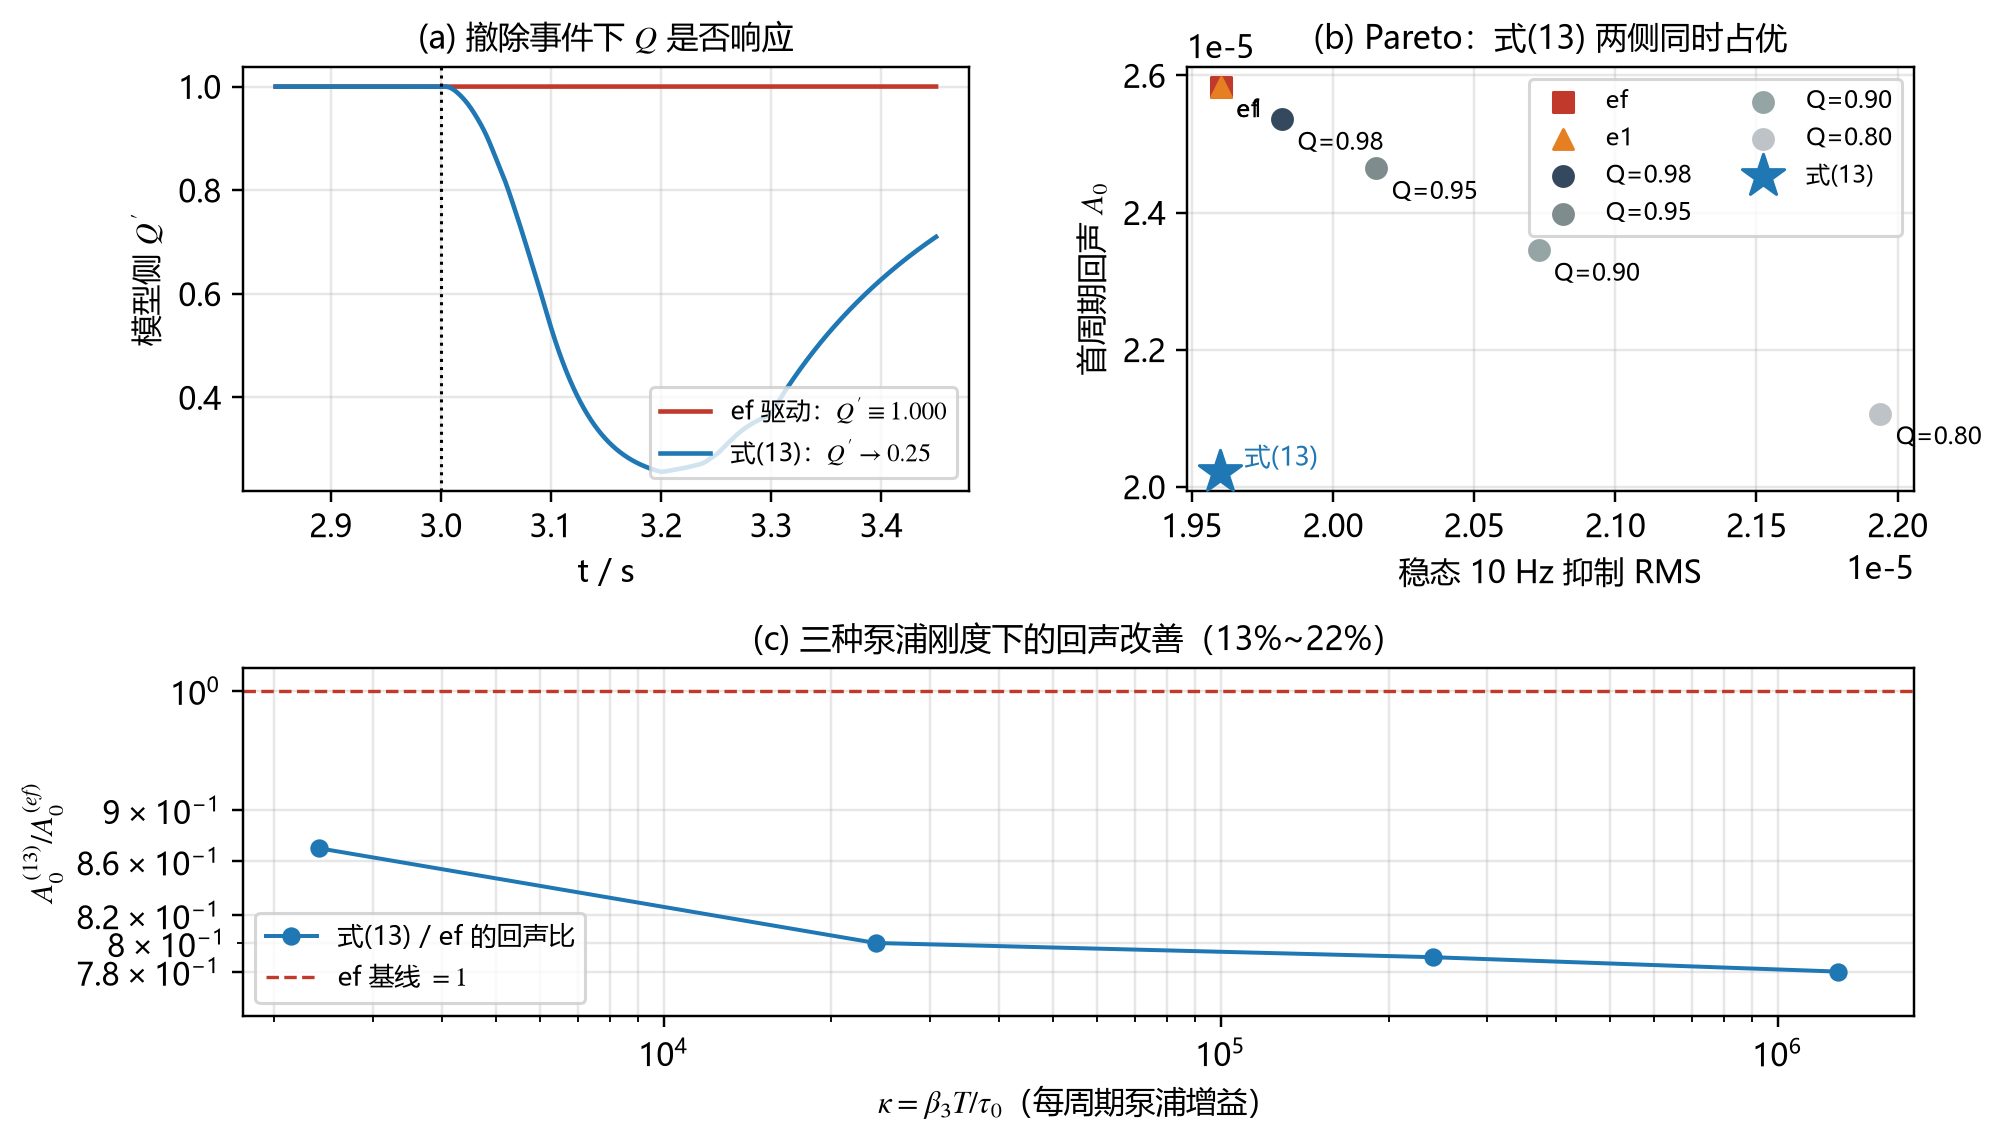
\includegraphics[width=0.92\textwidth]{fig_echo_q2.png}
\caption{\textbf{回声重影与记忆失配驱动}。(a) 撤除事件下 $Q'$ 是否响应：$e_f$ 驱动恒 $1.000$、式 \eqref{eq:mism} 降到 $0.25$；
(b) Pareto：式 \eqref{eq:mism}（星标）在稳态与回声两侧同时占优，静态 $Q$ 只能沿折中线滑动；
(c) 三种泵浦刚度下式 \eqref{eq:mism} 相对 $e_f$ 的回声比（$0.78\sim0.87$）。}
\label{fig:mism}
\end{figure}

% =====================================================================
\subsection{律 F：状态复位及其事件触发子类（ETSR）}\label{sec:etsr}
% =====================================================================
由 §\ref{sec:mism} 的时刻律 \eqref{eq:timing}，把"在事件附近清空状态"整理成一条可实现的律。
基础重复通道不变
\begin{equation}
  \tau_0\dot v+v=Q v(t-T)+\beta_3\st\!\Big(\frac{e_1}{\zeta}\Big),
  \label{eq:etsr-base}
\end{equation}
在其上叠加一个\emph{只在触发时刻作用}的状态复位算子
\begin{equation}
  \mathcal R_\alpha:\quad v(t_{\mathrm{trig}}^+)=\alpha v(t_{\mathrm{trig}}^-),\qquad
  v(t-T)\ \text{缓冲}\leftarrow\alpha v(t-T),
  \label{eq:etsr-reset}
\end{equation}
$\alpha=0$ 为清空（默认），$\alpha=-1$ 为反相复位（需已知事件为反相）。触发时刻
\begin{equation}
  t_{\mathrm{trig}}=t_e+\tau,\qquad
  \tau=\begin{cases}\tau_A\approx0 & \text{A：外部事件指示}\\[1mm]
  \tau_B=\tau_{\mathrm{det}}+\tau_{\mathrm{dec}} & \text{B：快包络检测}\end{cases}
  \label{eq:etsr-trig}
\end{equation}
其中 $\tau_{\mathrm{det}}\approx4\tau_f$（快包络 \eqref{eq:fastdet} 的上升时间）、$\tau_{\mathrm{dec}}=N\Delta t$ 为判决窗，
并要求冷却 $T_c$ 不小于一个扰动周期。

\begin{remark}[A 是上界，不是触发器]\label{rem:fa-oracle}
式 \eqref{eq:etsr-reset}--\eqref{eq:etsr-trig} 只规定"\textbf{何时}复位"，不规定"\textbf{如何}发现事件"——后者才是"事件触发"的定义。
\textbf{F-B 自带触发判据}（记忆失配 $D_m+g$，\S\ref{sec:fb-dilemma}，加冷却），无外部信息即可独立工作，故是\textbf{严格意义上的事件触发律，也是本文唯一可部署的律 F}；
\textbf{F-A 不含任何检测环节}，它把 $t_e$ 当作外部已知量（负载指令沿、驱动器状态位），只能作为"事件时刻精确已知"这一理想情形的\textbf{上界（oracle）}。
因此本文所有"F-A 优于 F-B"的数字都应读作\textbf{事件时刻精度的价值}，而不是两种律的优劣比较；B 档的 $88.9$ rpm 是\emph{本节一阶对象、旧 $e_1$ 包络检测器}的历史指标；真实对象定稿用 $D_m+g$，首周期 $6.20\pm2.65$\,rpm（\S\ref{sec:pmsm}），不可与 $88.9$ 混引。
\end{remark}

\noindent\textbf{两条支撑性质。}
\textbf{(P1) 不改变名义闭环}：$\mathcal R_\alpha$ 只作用于状态 $v$，不改 $Q,\beta_3,\tau_0$；
除复位瞬间外闭环与 §\ref{sec:uub} 的名义闭环完全一致，故其 UUB 界不变。
\textbf{(P2) 复位是有益跳变}：取 $V=\tfrac12v^2$，有 $V(t^+)=\alpha^2V(t^-)\le V(t^-)$（$|\alpha|\le1$），
故不破坏 §\ref{sec:uub} 的有界性论证；这也解释了为什么"清空状态"比"压低 $Q$"安全——
后者改的是\textbf{增益}，会同时削弱对现存周期分量的抑制（§\ref{sec:mism} 实测稳态 $46.7\to82.0$）。
此外首周期回声服从式 \eqref{eq:timing}：$A_0(0)=32.5$、$A_0(40\,\mathrm{ms})=88.9$、$A_0(\infty)=127.7$；
代价为复位后约一个周期的内模重建，冷却 $T_c=0.3$ s 时稳态 $10$ Hz 由 $46.7$ 升至 $48.7$（$+4.3\%$）。

\noindent\textbf{实现与边界}：A 档用外部事件指示直接调用复位（\texttt{memflush}）；
B 档定稿为记忆失配 $D_m>0.2$ 且 $g<0.05$、冷却 $0.3$\,s（\S\ref{sec:fb-dilemma}）；
旧包络开关仅保留回归，不得用于新结果。
真实对象 8 种子：首周期 $6.20\pm2.65$\,rpm（$-84.1\%$），D$+$F-B $5.69$（$-85.4\%$），
加载段 $0$ 误触发、跌落/稳态/电流不劣化；F-A 立即复位不是上界（$19.14$ 对延时 $20$\,ms 的 $2.73$）。
“$\tau$ 越小收益越大”只在一阶对象上成立，真实对象最优在 $20$--$25$\,ms（\S\ref{sec:pmsm}）。

\begin{figure}[htbp]\centering
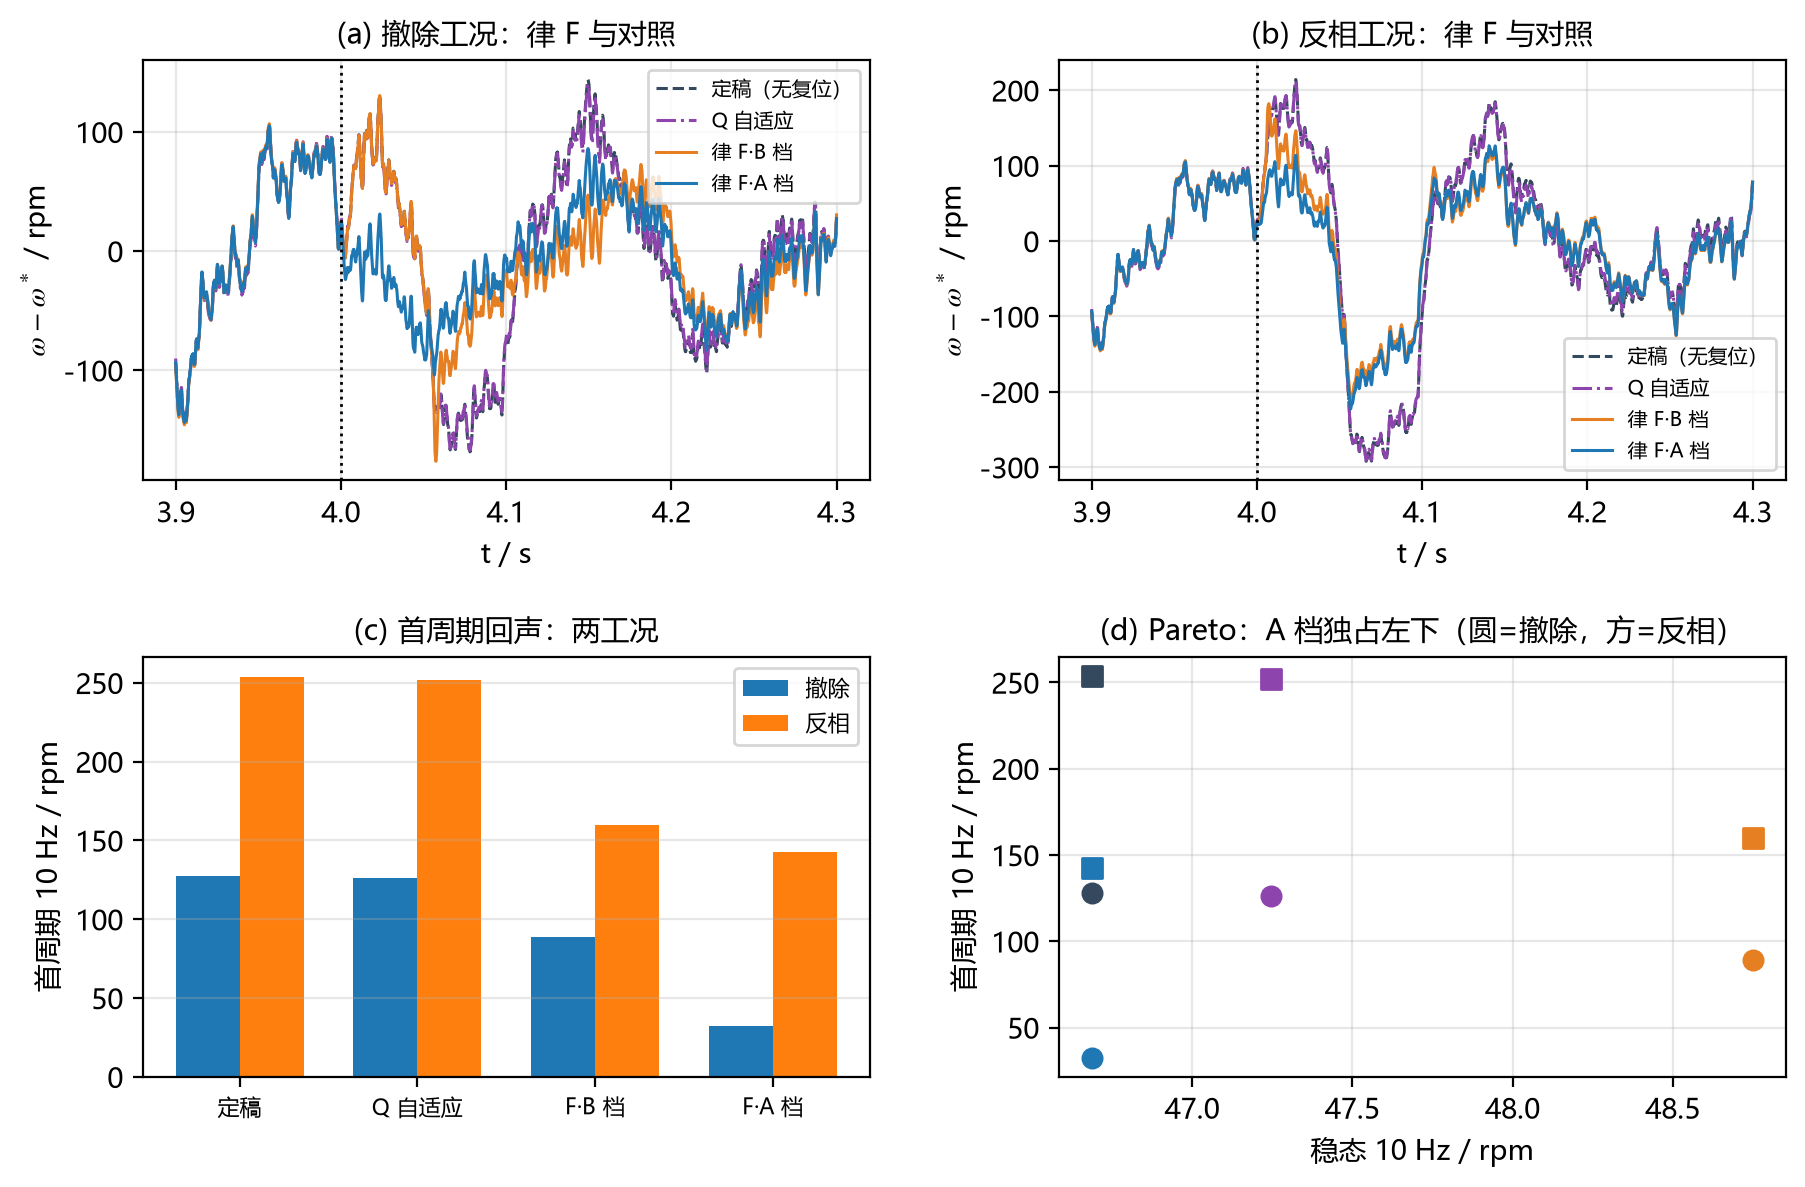
\includegraphics[width=0.86\textwidth]{fig_echo_lawF.png}
\caption{\textbf{律 F 与三类对照的对比}（同一工况、同一噪声实现；圆/方分别对应撤除/反相）。
(a)(b) 两种工况下的转速误差；(c) 首周期 $10$ Hz 回声（两工况并列）；
(d) Pareto：横轴为稳态 $10$ Hz、纵轴为首周期回声——A 档（事件时刻复位）独占左下（$46.7/32.5$），
B 档次之（$48.7/88.9$），而 $Q$ 自适应几乎与定稿重合（$47.2/126.1$ 对 $46.7/127.7$）。
律 F 的两档把"复位时刻"这一唯一变量显式化了。}
\label{fig:echo-lawF}
\end{figure}

\section{本版（带通）律的可证结论}\label{sec:stab}
\subsection{结构前提：驱动有界性}\label{sec:newpremise}
本版驱动 $D=w_f-w_l$（\eqref{eq:bpw}）是\emph{带通}，其"非负 / 周期零均值"均不成立，故不能沿用旧放缩。下面两条引理给出对本版驱动直接成立的前提，\textbf{证明只用到 $\phi$ 的 $1$-Lipschitz 性与滤波核为凸组合}，与驱动的符号结构无关。
\begin{lemma}[零均值带通驱动的有界性]\label{lem:Dbound}
设 $M_t:=\sup_{s\le t}\ef^{2}(s)<\infty$、$\varepsilon>0$、$c>0$、$\tau_f^{w},\tau_l^{w}>0$，实参取零均值形式 \eqref{eq:phi-x}。则
\begin{equation}
  |D(t)|\le\min\Bigl\{2,\;\frac{2M_t}{\varepsilon}\Bigr\},\qquad\text{从而}\qquad
  |D_Q(t)|=|D(t)|.
  \label{eq:Dbound}
\end{equation}
\emph{证明.} 记 $x=\dfrac{\ef^{2}-E_o}{E_o+\varepsilon}$，则 $\phi(0)=0$ 且 $\phi(\cdot,c)$ 为 $1$-Lipschitz，故 $|w|=|\phi(x,c)|\le|x|$。
又 $|x|\le\dfrac{|\ef^{2}|+E_o}{E_o+\varepsilon}\le1+\dfrac{|\ef^{2}|}{E_o+\varepsilon}\le1+\dfrac{M_t}{\varepsilon}$；
且 $|x|\le\dfrac{|\ef^{2}-E_o|}{\varepsilon}\le\dfrac{M_t}{\varepsilon}$（用 $E_o\ge0$）。两式取小即得 $|w|\le\min\{1,M_t/\varepsilon\}$。
一阶低通的核 $\frac{1}{\tau^{w}}e^{-t/\tau^{w}}$ 非负、积分为 $1$，故 $w_f,w_l$ 均为 $w$ 的历史凸组合，各自落在 $[\inf w,\sup w]$ 内，于是 $|D|=|w_f-w_l|\le2\sup|w|$。
因 $D_Q=D$（\eqref{eq:shared-D}），驱动界即为 $Q$ 通道的界。$\square$
\end{lemma}
\begin{remark}[零均值实参在分析上的两重好处]\label{rem:zero-mean}
\textbf{(i) 界更紧且与 $\varepsilon$ 解耦}：实参取 $\ef^{2}/(E_o+\varepsilon)$（恒正）时只能得到 $|D|\le2M_t/\varepsilon$，$\varepsilon\to0$ 时界发散；取零均值形式后有 $|D|\le2$，\textbf{对一切 $\varepsilon>0$ 一致成立}。
\textbf{(ii) 平衡点回到可用区}：恒正实参使 $w$ 恒正、$\overline{D}>0$，$Q$ 被单向压到底（实测动作仅 $\pm1.5\times10^{-4}$）；零均值实参使 $\overline{D}\approx0$，$Q$ 的平衡点回到 $1$ 附近，$Q$ 才具备调节能力。
\end{remark}
\begin{remark}[闭环一致有界性的归并与仍开放的问题]\label{rem:robust}
\textbf{(已归并)} 名义闭环的 UUB 与"含 $Q/B/D$ 调度"的推论见 §\ref{sec:uub}：$v$ 通道自持有界（界 $\beta_3/(1-Q_0)$，与 $e_1$ 大小无关），
ESO 误差与跟踪误差的界显式依赖 $(\beta_3,Q_0,\omega_o,k_p,b,b_0,H)$；且因 $g\in[0,1)$、$\kappa\ge0$ 使增益只增不减，\textbf{名义界即调度闭环的界}。
\textbf{(仍开放)} (i) 随机噪声（电流/负载噪声）不属该确定性框架，其定量影响由敏感性一节单独量化；
(ii) 三个界都是\emph{保守上界}（与仿真实测相差 $10^{2}\sim10^{5}$ 倍），收紧界需更强的结构信息。
\end{remark}
\subsection{名义闭环的一致有界性（UUB）：完整证明}\label{sec:uub}
\textbf{设定}：名义闭环指 $\tau\equiv\tau_0$、$Q\equiv Q_0$ 固定、调度全关（$g\equiv0$）的闭环。
记 $e_1=x_1-z_1$、$e_2=x_2-z_2$，$x_2$ 为含输入失配的扩张状态，$\dot x_2=:h$。
\textbf{假设}：(A1) $|h(t)|\le H$；(A2) $b,b_0,k_p,\omega_o,\tau_0,\zeta>0$、$Q_0\in(0,1)$、$\beta_3\ge0$；(A3) $r$ 为常数、$d$ 有界。

\noindent\textbf{引理 1（重复通道自持 UUB）}：由 $|\tanh(\cdot)|\le1$，重复通道输入满足
$|Q_0v(t-T)+\beta_3\tanh(e_1/\zeta)|\le Q_0\bar V+\beta_3$（$\bar V:=\sup_{[t-T,t]}|v|$）；
一阶低通在 $|w|\le W$ 下满足 $|v(t)|\le W+(|v(0)|-W)e^{-t/\tau_0}$，逐周期迭代得
\begin{equation}
\limsup_{t\to\infty}|v(t)|\le\bar v:=\frac{\beta_3}{1-Q_0}.
\label{eq:uub-v}
\end{equation}
\emph{关键}：该界\textbf{与 $e_1$ 的大小无关}（因 $\tanh$ 有界），故 $v$ 通道"自持"，不构成代数环。

\noindent\textbf{引理 2（ESO 误差 UUB）}：ESO 误差动态为 $\dot e_1=-2\omega_o e_1+e_2-v$、$\dot e_2=-\omega_o^{2}e_1+h$。
取尺度化坐标 $\xi=[e_1,\ e_2/\omega_o]^{\!\top}$，则 $\dot\xi=\omega_o A_0\xi+w_d$，
$A_0=\left[\begin{smallmatrix}-2&1\\-1&0\end{smallmatrix}\right]$（特征值 $-1$ 二重），$w_d=[-v,\ h/\omega_o]^{\!\top}$。
解 $A_0^{\!\top}P_0+P_0A_0=-I$ 得 $P_0=\left[\begin{smallmatrix}0.5&-0.5\\-0.5&1.5\end{smallmatrix}\right]\succ0$（特征值 $0.191/1.809$），$\|P_0B_0\|_F=\sqrt3$。
取 $V=\xi^{\!\top}P_0\xi$ 得 $\dot V\le-\omega_o\|\xi\|^{2}+2\sqrt3\,\|\xi\|\,\|w_d\|$，故
\begin{equation}
\limsup_{t\to\infty}\|\xi(t)\|\le\frac{2\sqrt3}{\omega_o}\sqrt{\bar v^{2}+\bigl(H/\omega_o\bigr)^{2}} .
\label{eq:uub-eso}
\end{equation}

\noindent\textbf{引理 3（跟踪误差 UUB）}：令 $\sigma=r-y$，由 $\dot y=\frac{b}{b_0}(k_p\sigma-z_2-v)+d$ 得
$\sigma\dot\sigma\le-\frac{bk_p}{b_0}\sigma^{2}+|\sigma|\bigl(|d|+\frac{b}{b_0}(|z_2|+\bar v)\bigr)$，而 $z_2=x_2-e_2$ 有界，故
\begin{equation}
\limsup_{t\to\infty}|\sigma(t)|\le\frac{b_0}{bk_p}\Bigl(\sup|d|+\frac{b}{b_0}\bigl(\sup|x_2|+\bar v\bigr)\Bigr).
\label{eq:uub-track}
\end{equation}

\noindent\textbf{定理（名义闭环 UUB）}：在 (A1)--(A3) 下，式 \eqref{eq:uub-v}--\eqref{eq:uub-track} 同时成立，
闭环全部信号一致最终有界，界\textbf{显式}依赖 $(\beta_3,Q_0,\omega_o,k_p,b,b_0,H)$。
\emph{注}：(a) 本例回代：$\beta_3=2000$、$Q_0=0.98\Rightarrow\bar v=10^{5}$、$\omega_o=40$；三个界都是\textbf{保守上界}
（仿真实测 $|v|\approx4.5\times10^{2}$、$|e_1|\approx0.05$，相差 $10^{2}\sim10^{5}$ 倍），定量行为以仿真为准；
(b) (A1) 的 $h$ 含 $\dot u$ 项，而 $u$ 由有界的 $z_2,v$ 构成，故 $h$ 的有界性由前述界隐式给出（有限）。

\noindent\textbf{推论（含 $Q/B/D$ 调度）}：$g=\bar e_1^{2}/(\bar e_1^{2}+\varepsilon_g^{2})\in[0,1)$ 由构造保证，$\kappa_p,\kappa_B\ge0$，
故 $k_p^{\rm eff}=k_p(1+\kappa_pg)\ge k_p$、$\omega_o^{\rm eff}=\omega_o(1+\kappa_Bg)\ge\omega_o$；
式 \eqref{eq:uub-eso}\eqref{eq:uub-track} 的界对 $(\omega_o,k_p)$ \textbf{单调不增}，故\emph{名义界即调度闭环的界}：
\textbf{调度可证地不放大一致最终界}。这与"调度放大噪声本底"的仿真事实不矛盾——噪声不在本确定性框架内，由敏感性一节单独量化。
\section{数值验证（沿真实轨迹逐条核对）}\label{sec:verify}
% =====================================================================
轨迹来源：\texttt{nk\_trace.npz}（本版带通律，$\gamma=3$、$\sigma_1^{\mathrm{code}}=10^{5}$、$\sigma_2=5$、$\mu=0.03$、$q'_{\max}=1.0$、$\tau'\in[0.2,5]$，$c_1=c_2=0$（\emph{本档未启用 $\phi$ 压缩与驱动死区}）、$\varepsilon=6.5$、$\Delta t=2\times10^{-5}$ s，$5\times10^{5}$ 步）。
\begin{center}
\footnotesize
\begin{tabular}{@{}llll@{}}
\toprule
断言 & 来源 & 数值 & 判定\\
\midrule
$|D|\le\min\{2,\;2M_t/\varepsilon\}$ & 引理 \ref{lem:Dbound} & $|D|_{\max}=2.97$ & \pv{实测}\\
$v$ 通道自持 UUB & 引理（§\ref{sec:uub}） & $|v|\le\beta_3/(1-Q_0)$ & \pv{已证}\\
$Q'\in[0.2,1.0]$ & \eqref{eq:clip-model} & $[0.2532,\,0.9991]$，未触界 & \pv{实测}\\
$Q'\in[0.2,1.0]$（模型侧） & \eqref{eq:clip-model} & $[0.2532,\,0.9991]$，未触界 & \pv{实测}\\
\bottomrule
\end{tabular}
\end{center}
\textbf{说明}：表中各项均取自同一次运行的真实轨迹；$z_2$ 的直流分量见注 \ref{rem:z2dc}，$Q$ 的取值与限幅见 \S\ref{sec:qch}。

\section{PMSM 转速环：真实逆变器对象（2026-10-19 定稿）}\label{sec:pmsm}
\textbf{口径声明}：本节对象严格为\textbf{三相 PWM 逆变器 + PMSM}，不再使用一阶/降阶电流环等效；
旧对象（一阶电流环、$T_s=10\,\mu$s 单速率）的数值已从正文删除，不得再引用。
\S\ref{sec:model}--\S\ref{sec:verify} 的证明仍在标幺一阶模型上给出，用于结构性质；
\textbf{数值与工程结论以本节真实对象为准}。

\subsection{对象：三相 PWM 逆变器 + PMSM}
模型为 \texttt{pmsm\_inv\_sim}：
\begin{center}\footnotesize
\begin{tabular}{@{}llll@{}}
\toprule
项目 & 取值 & 项目 & 取值\\
\midrule
母线 / 开关频率 & $60$\,V / $10$\,kHz & 死区 / 器件压降 & $2\,\mu$s / $0.9$\,V\\
相电感 / 电阻 & $L_d=L_q=0.57$\,mH / $0.175\,\Omega$ & 磁链 / 极对数 & $\psi_f=0.01683$\,Wb / $4$\\
转动惯量 & $J=1.89\times10^{-5}$ kg$\cdot$m$^2$ & 电流环带宽 & $f_{ci}=2$\,kHz\\
重复通道 & $\beta_3=4000$、$\tau_0=20$\,ms & 速度环 & $k_p=75.36$、$\omega_o=500$\\
dq 采样噪声 & $\pm0.2$\,A（$10$\,kHz） & 编码器 & $2500$ PPR（$4\times$）\\
负载噪声 / 转速噪声 & $0.025$\,N$\cdot$m / $6$\,rpm（$1\%$） & 积分步长 & $2\,\mu$s（$8$\,s 轨迹）\\
\bottomrule
\end{tabular}
\end{center}
逆变器按中心对齐 PWM 比较、死区平均电压误差 $\mp V_{dc}T_d/T_{pwm}$、器件压降与导通电阻建模；
电机侧 $L_d,L_q$ 与反电动势 $\omega_e\psi_f$ 显式进入 dq ODE；相电流由 dq 反变换得到，
逆变器电压再 Park 回 dq。工况：$0$--$2$\,s 空载，$2$\,s 加载 $0.50$ 额定，$2$--$6$\,s 叠加
$10$\,Hz 不对中簇（$A=0.30$），$6$\,s 零交越撤除；$8$\,s 轨迹，$8$ 个种子。

\noindent\textbf{三档噪声工况}（2026-10-20 定义；本文未注明时一律为标准工况）：
\begin{center}\footnotesize
\begin{tabular}{@{}lccc@{}}
\toprule
工况 & 转速噪声 & dq 电流噪声 & 负载转矩噪声\\
\midrule
实验室 & $\le0.5\%$（$3$\,rpm） & $\le0.1$\,A & $\le0.01$\,N$\cdot$m\\
标准（默认） & $1\%$（$6$\,rpm） & $0.2$\,A & $0.025$\,N$\cdot$m\\
恶劣 & $>2\%$（取 $2.5\%$，$15$\,rpm） & $>0.3$\,A（取 $0.4$） & $>0.05$\,N$\cdot$m（取 $0.06$）\\
\bottomrule
\end{tabular}
\end{center}

\begin{figure}[htbp]\centering
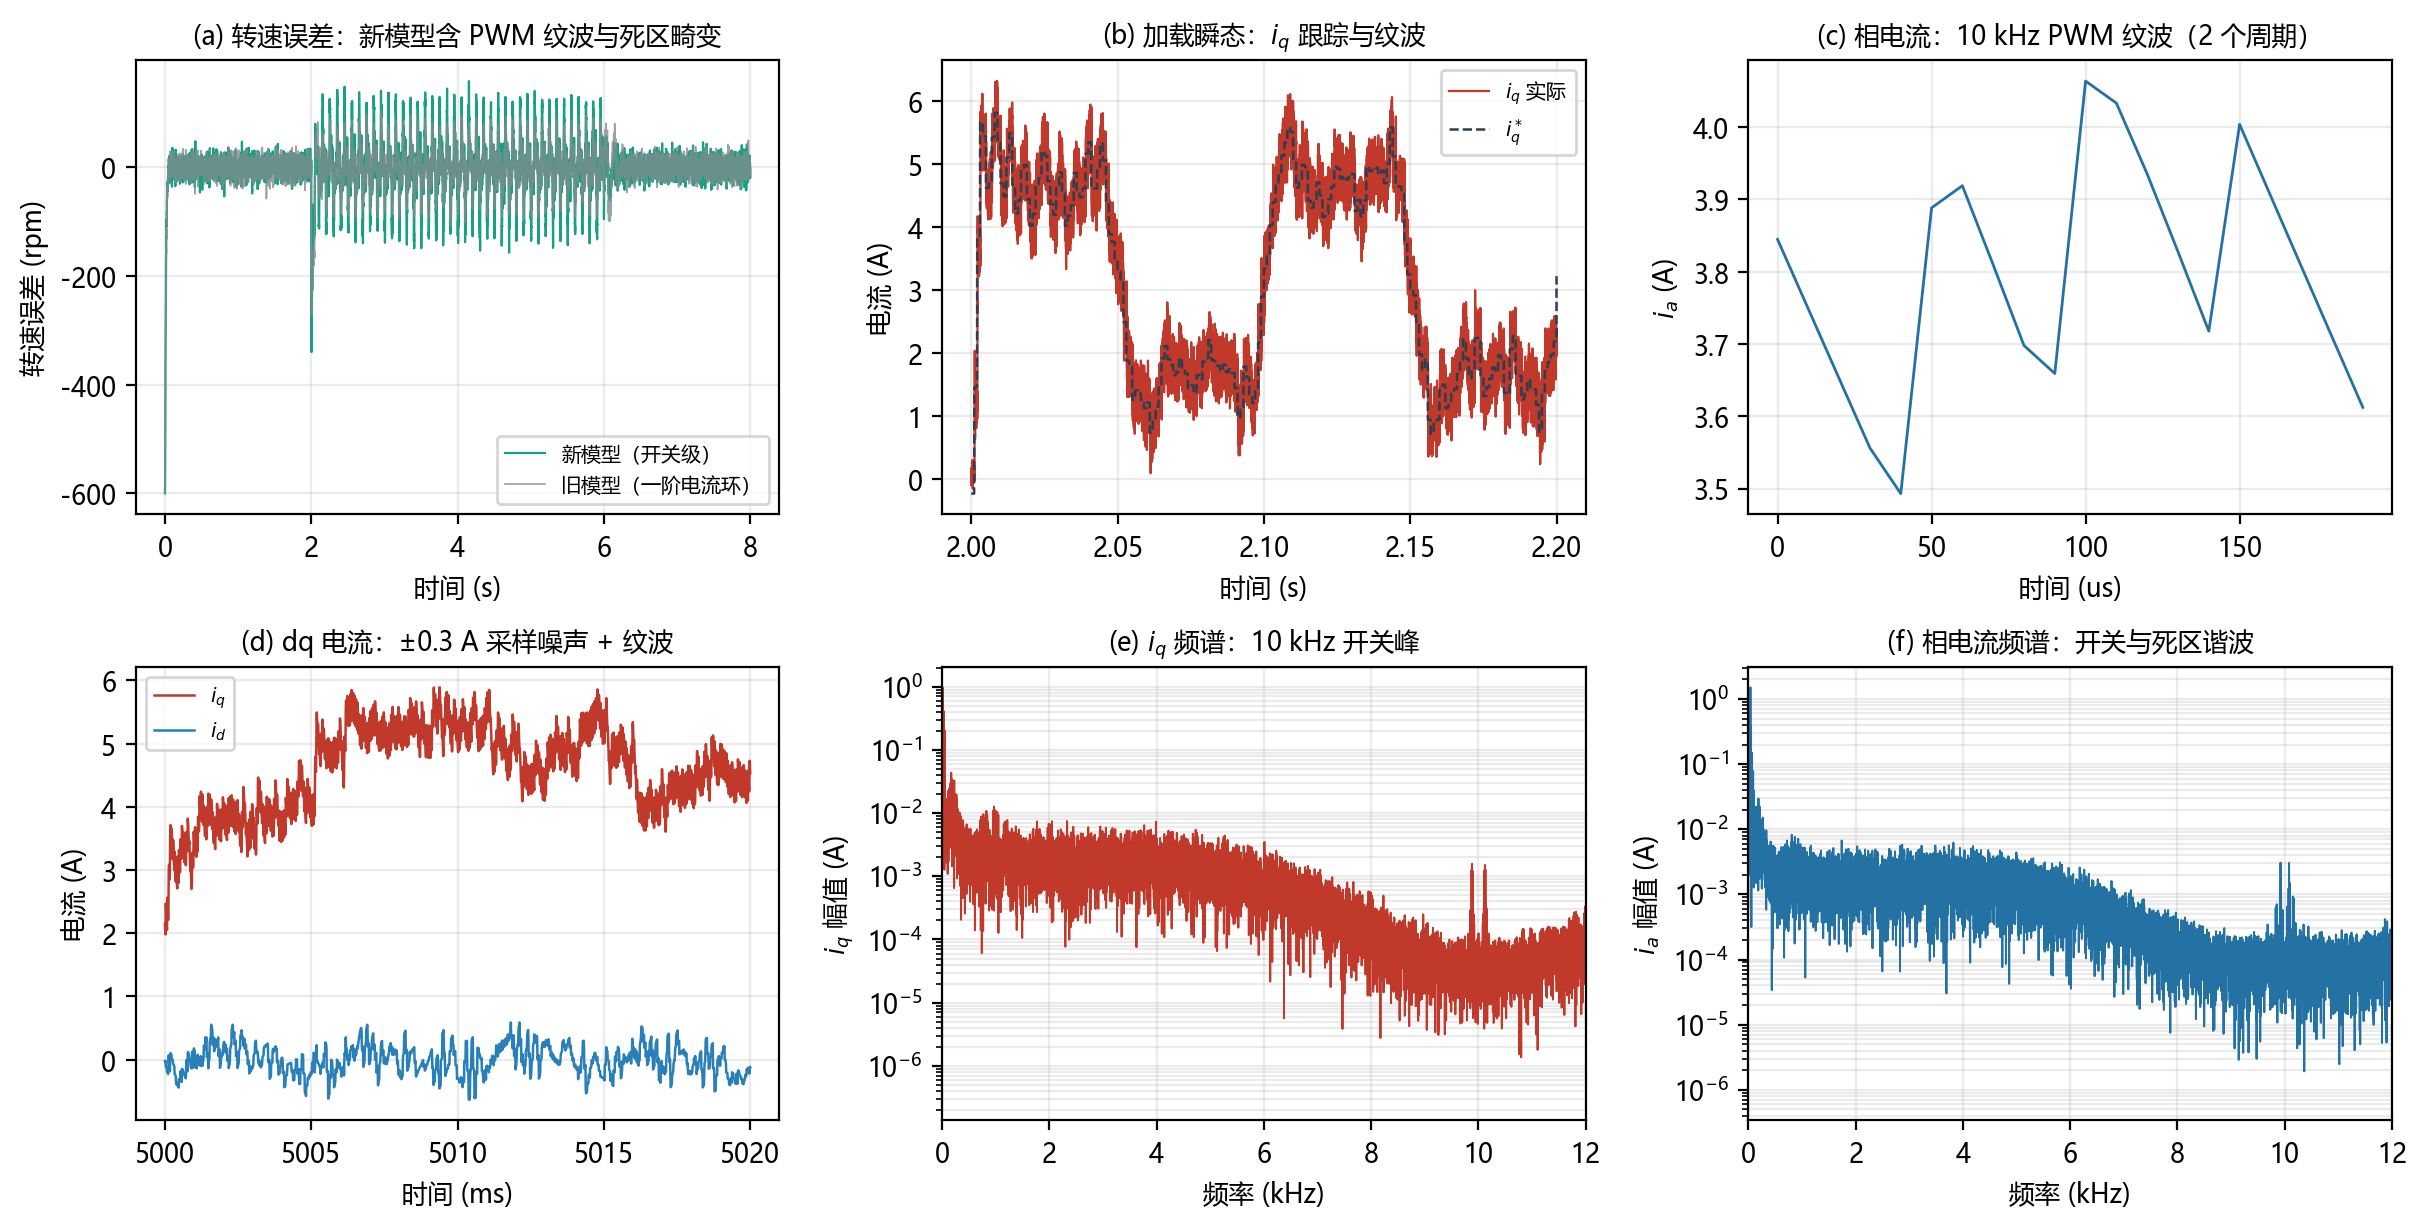
\includegraphics[width=0.99\textwidth]{fig_inv_demo.png}
\caption{\textbf{真实逆变器对象的电流}。(a) 转速误差；(b) 加载瞬态 $i_q/i_q^*$；
(c) 相电流 $200\,\mu$s 放大（$10$\,kHz PWM 纹波）；(d) dq 电流 $20$\,ms 放大（$\pm0.2$\,A 采样噪声/纹波）；
(e)(f) $i_q$/相电流频谱（$10$\,kHz 开关峰与死区谐波）。}
\label{fig:inv-demo}
\end{figure}

\subsection{稳定性重调：$220$\,Hz 极限环}
旧 dq 对象的 $\tau_0=5$\,ms、$\beta_3=2000$ 在真实对象上出现 $220$\,Hz 极限环
（$i_q$ 标准差 $2.29$\,A、转速标准差 $81$\,rpm）：重复通道的 $1/\tau_0\approx200$\,Hz 极点
叠加 PWM/电流环延迟，相位裕度不足。$4$\,s 周期负载实测：

\begin{center}\footnotesize
\begin{tabular}{@{}lccc@{}}
\toprule
配置 & 带载 RMS & 撤除后 RMS & $i_q$ std\\
\midrule
无 RC & $258.05$ & $17.98$ & $1.68$\\
$\beta_3=2000,\ \tau_0=20$\,ms & $92.55$ & $13.86$ & $1.60$\\
$\beta_3=4000,\ \tau_0=20$\,ms, $f_{ci}=2$\,kHz & $\mathbf{56.03}$ & $\mathbf{12.91}$ & $1.58$\\
$\beta_3=4000,\ \tau_0=10$\,ms & $59.20$ & $58.60$（不稳） & $2.10$\\
\bottomrule
\end{tabular}
\end{center}
定稿取 $\tau_0=20$\,ms、$\beta_3=4000$、$f_{ci}=2$\,kHz；$\tau_0$ 不能再压到 $10$\,ms。

\subsection{四档算法：8 种子}
\begin{center}\footnotesize
\begin{tabular}{@{}lcccc@{}}
\toprule
配置 & 首周期 $10$\,Hz & 加载跌落 & 稳态 $7$--$8$\,s & $7$--$8$\,s 复位\\
\midrule
Base & $39.05\pm0.47$ & $-337.23\pm3.83$ & $18.77\pm0.12$ & 0\\
律 D & $36.36\pm0.47$（$-6.9\%$） & $-331.39\pm4.83$（$-1.7\%$） & $18.70\pm0.16$ & 0\\
F-B（$D_m+g$） & $\mathbf{6.20\pm2.65}$（$-84.1\%$） & $-337.17\pm4.64$ & $18.76\pm0.15$ & $3.1$\\
律 D $+$ F-B & $\mathbf{5.69\pm2.78}$（$-85.4\%$） & $-330.46\pm3.89$（$-2.0\%$） & $18.76\pm0.16$ & $3.2$\\
\bottomrule
\end{tabular}
\end{center}
读数：(i) 律 D 仍 Pareto，但收益远小于旧对象（跌落仅 $-1.7\%$、回声 $-6.9\%$）：
真实跌落由 PWM/电流环延迟、死区与噪声共同决定，抬 $k_p$ 能顶住的部分被压缩；
(ii) F-B 用记忆失配 $D_m$ 与 $g$ 门控，$8/8$ 种子命中（首触发 $6.011$--$6.02$\,s），
加载段 $0$ 次误触发；与律 D 组合 $-85.4\%$；
(iii) 残余为 $7$--$8$\,s 每秒约 $3$ 次复位，稳态 $18.76$ 对 Base $18.77$（$6$\,rpm 噪声抬高基数，四者差 $<0.1$）；
(iv) 旧包络比值在同一对象上 $k=1.8$ 零触发、$k=1.3$ 虽命中但跌落 $-334\to-380$，
已否决（\S\ref{sec:fb-dilemma}）。

\begin{figure}[htbp]\centering
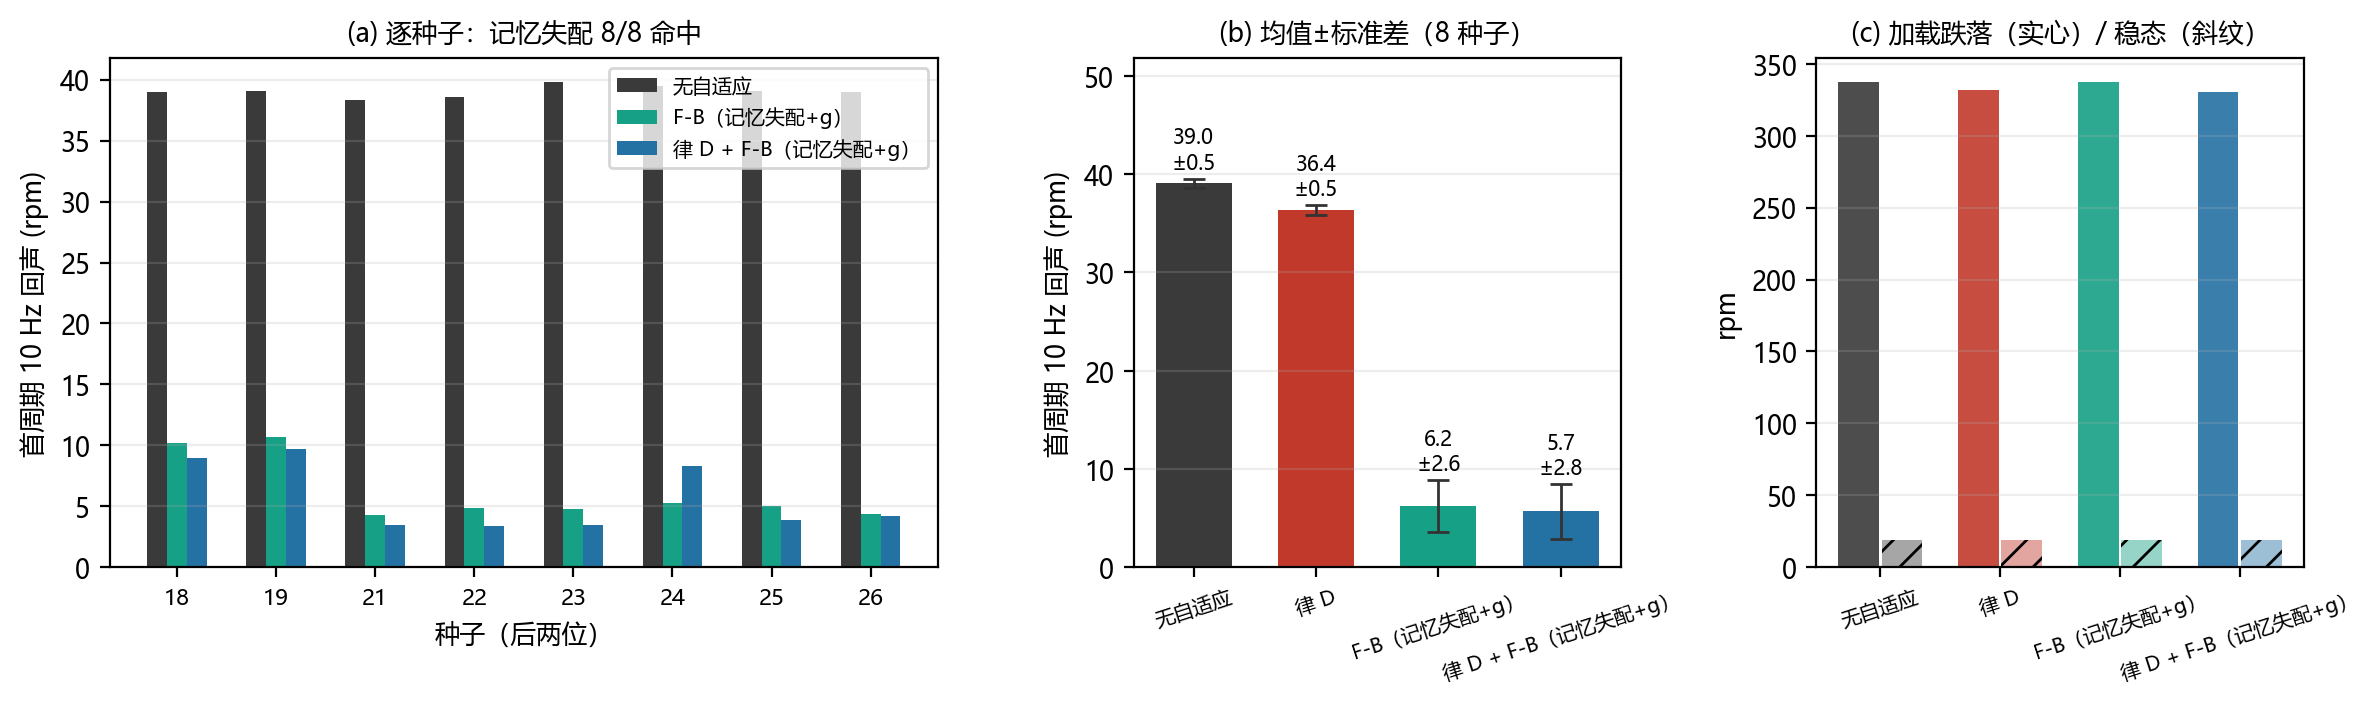
\includegraphics[width=0.99\textwidth]{fig_inv_mism.png}
\caption{\textbf{记忆失配 F-B 的 8 种子结果}。(a) 逐种子首周期 $10$\,Hz：$8/8$ 命中；
(b) 均值$\pm$标准差；(c) 加载跌落与稳态：F-B 不劣化，D$+$F-B 略有改善。}
\label{fig:inv-mism}
\end{figure}

\subsection{实验室工况：律 D 与 F-B}\label{sec:lab}
按三档中的实验室工况（转速 $0.5\%=3$\,rpm、电流 $0.1$\,A、负载 $0.01$\,N$\cdot$m）重跑
$8$ 种子；标准工况表保留，二者不混引。

\begin{center}\footnotesize
\begin{tabular}{@{}lcccc@{}}
\toprule
配置 & 首周期 $10$\,Hz & 加载跌落 & 稳态 $7$--$8$\,s & $7$--$8$\,s 复位\\
\midrule
Base & $37.49\pm0.17$ & $-336.19\pm2.66$ & $8.45\pm0.11$ & 0\\
律 D & $35.38\pm0.19$（$-5.6\%$） & $\mathbf{-327.81\pm1.00}$（$-2.5\%$） & $8.33\pm0.06$ & 0\\
F-B（$D_m+g$） & $\mathbf{6.44\pm1.73}$（$-82.8\%$） & $-342.21\pm19.00$ & $8.52\pm0.16$ & $3.1$\\
律 D $+$ F-B & $\mathbf{4.94\pm1.93}$（$-86.8\%$） & $-346.73\pm28.14$ & $8.45\pm0.14$ & $3.2$\\
\bottomrule
\end{tabular}
\end{center}
读数：实验室工况下回声仍由 F-B 主导（$6.44$、D$+$F-B $4.94$，律 D 仅 $35.38$）；
但\textbf{跌落并不随噪声降低而变干净}：律 D 为 $-327.81\pm1.00$，F-B 为 $-342.21\pm19.00$
（种子 023 达 $-388.8$），D$+$F-B 为 $-346.73\pm28.14$（种子 025 达 $-385.1$）——低噪声下
$g$ 门控在加载瞬态仍可能短暂失守，造成误复位与跌落种子离散。故实验室工况的结论是：
\textbf{律 D 管跌落更稳，F-B 管回声更强；F-B 的跌落离群需带载门控修正}（实验性
$|i_q|>1.5$\,A 门控可抑制，1 种子实测，未 8 种子定稿）。

\begin{figure}[htbp]\centering
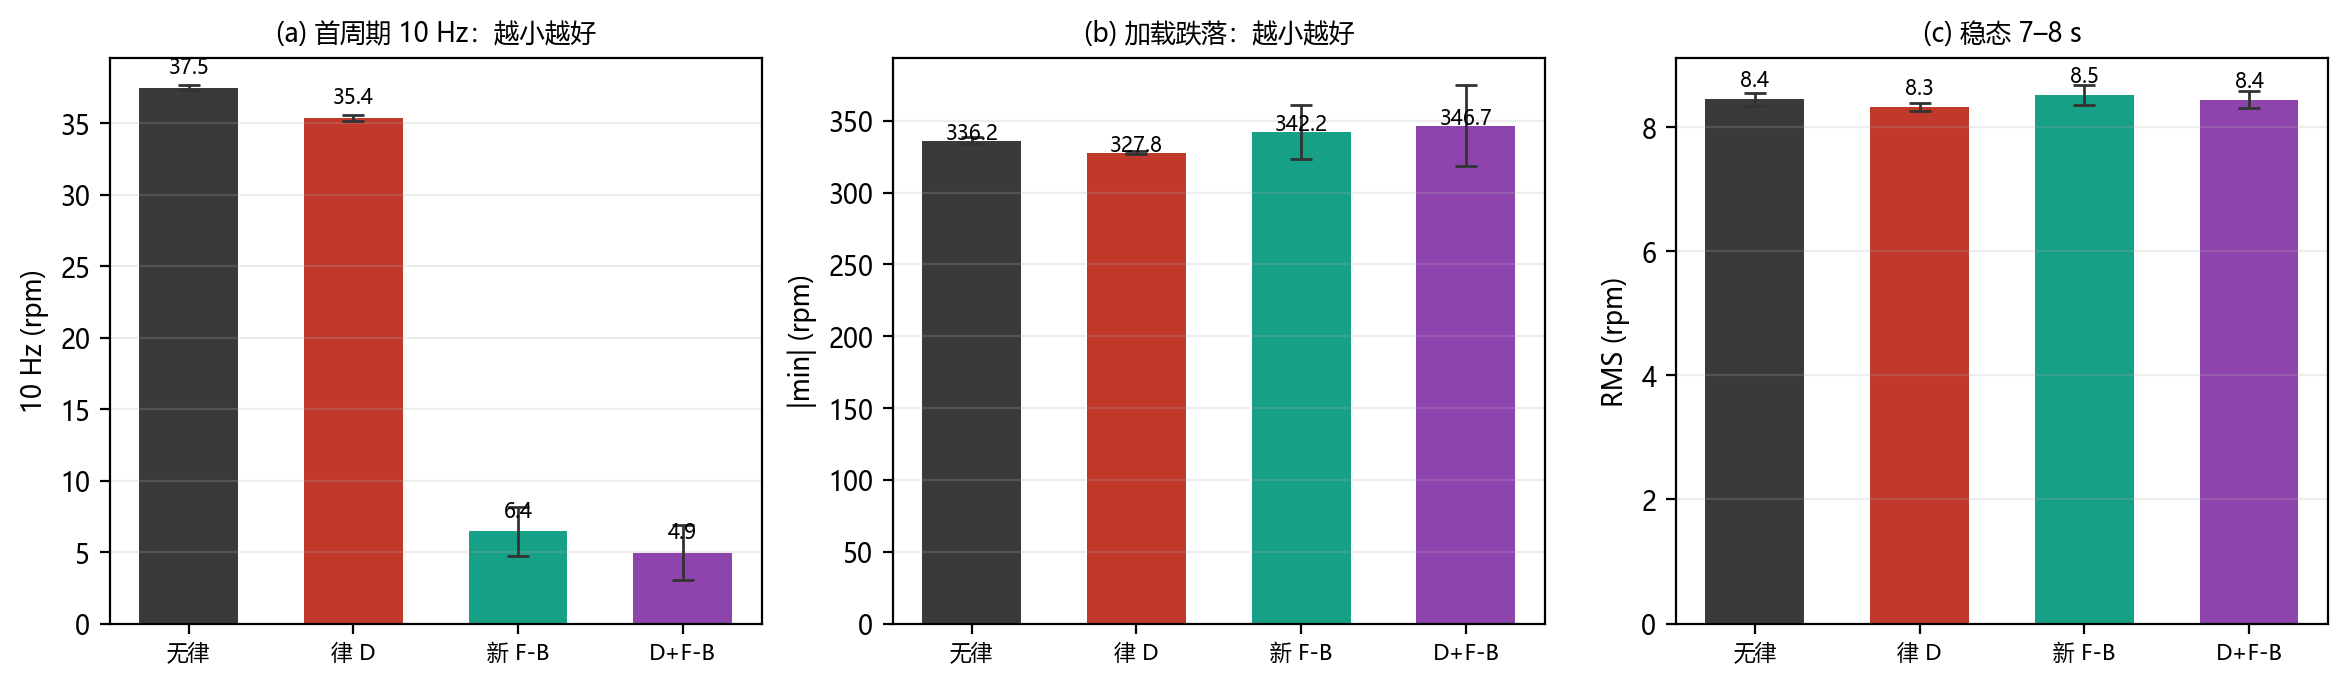
\includegraphics[width=0.99\textwidth]{fig_inv_lab.png}
\caption{\textbf{实验室工况（$3$\,rpm / $0.1$\,A / $0.01$\,N$\cdot$m）}：
(a) 首周期 $10$\,Hz；(b) 加载跌落；(c) 稳态。F-B 回声最低，但跌落误差棒显著大于律 D。}
\label{fig:inv-lab}
\end{figure}

\begin{figure}[htbp]\centering
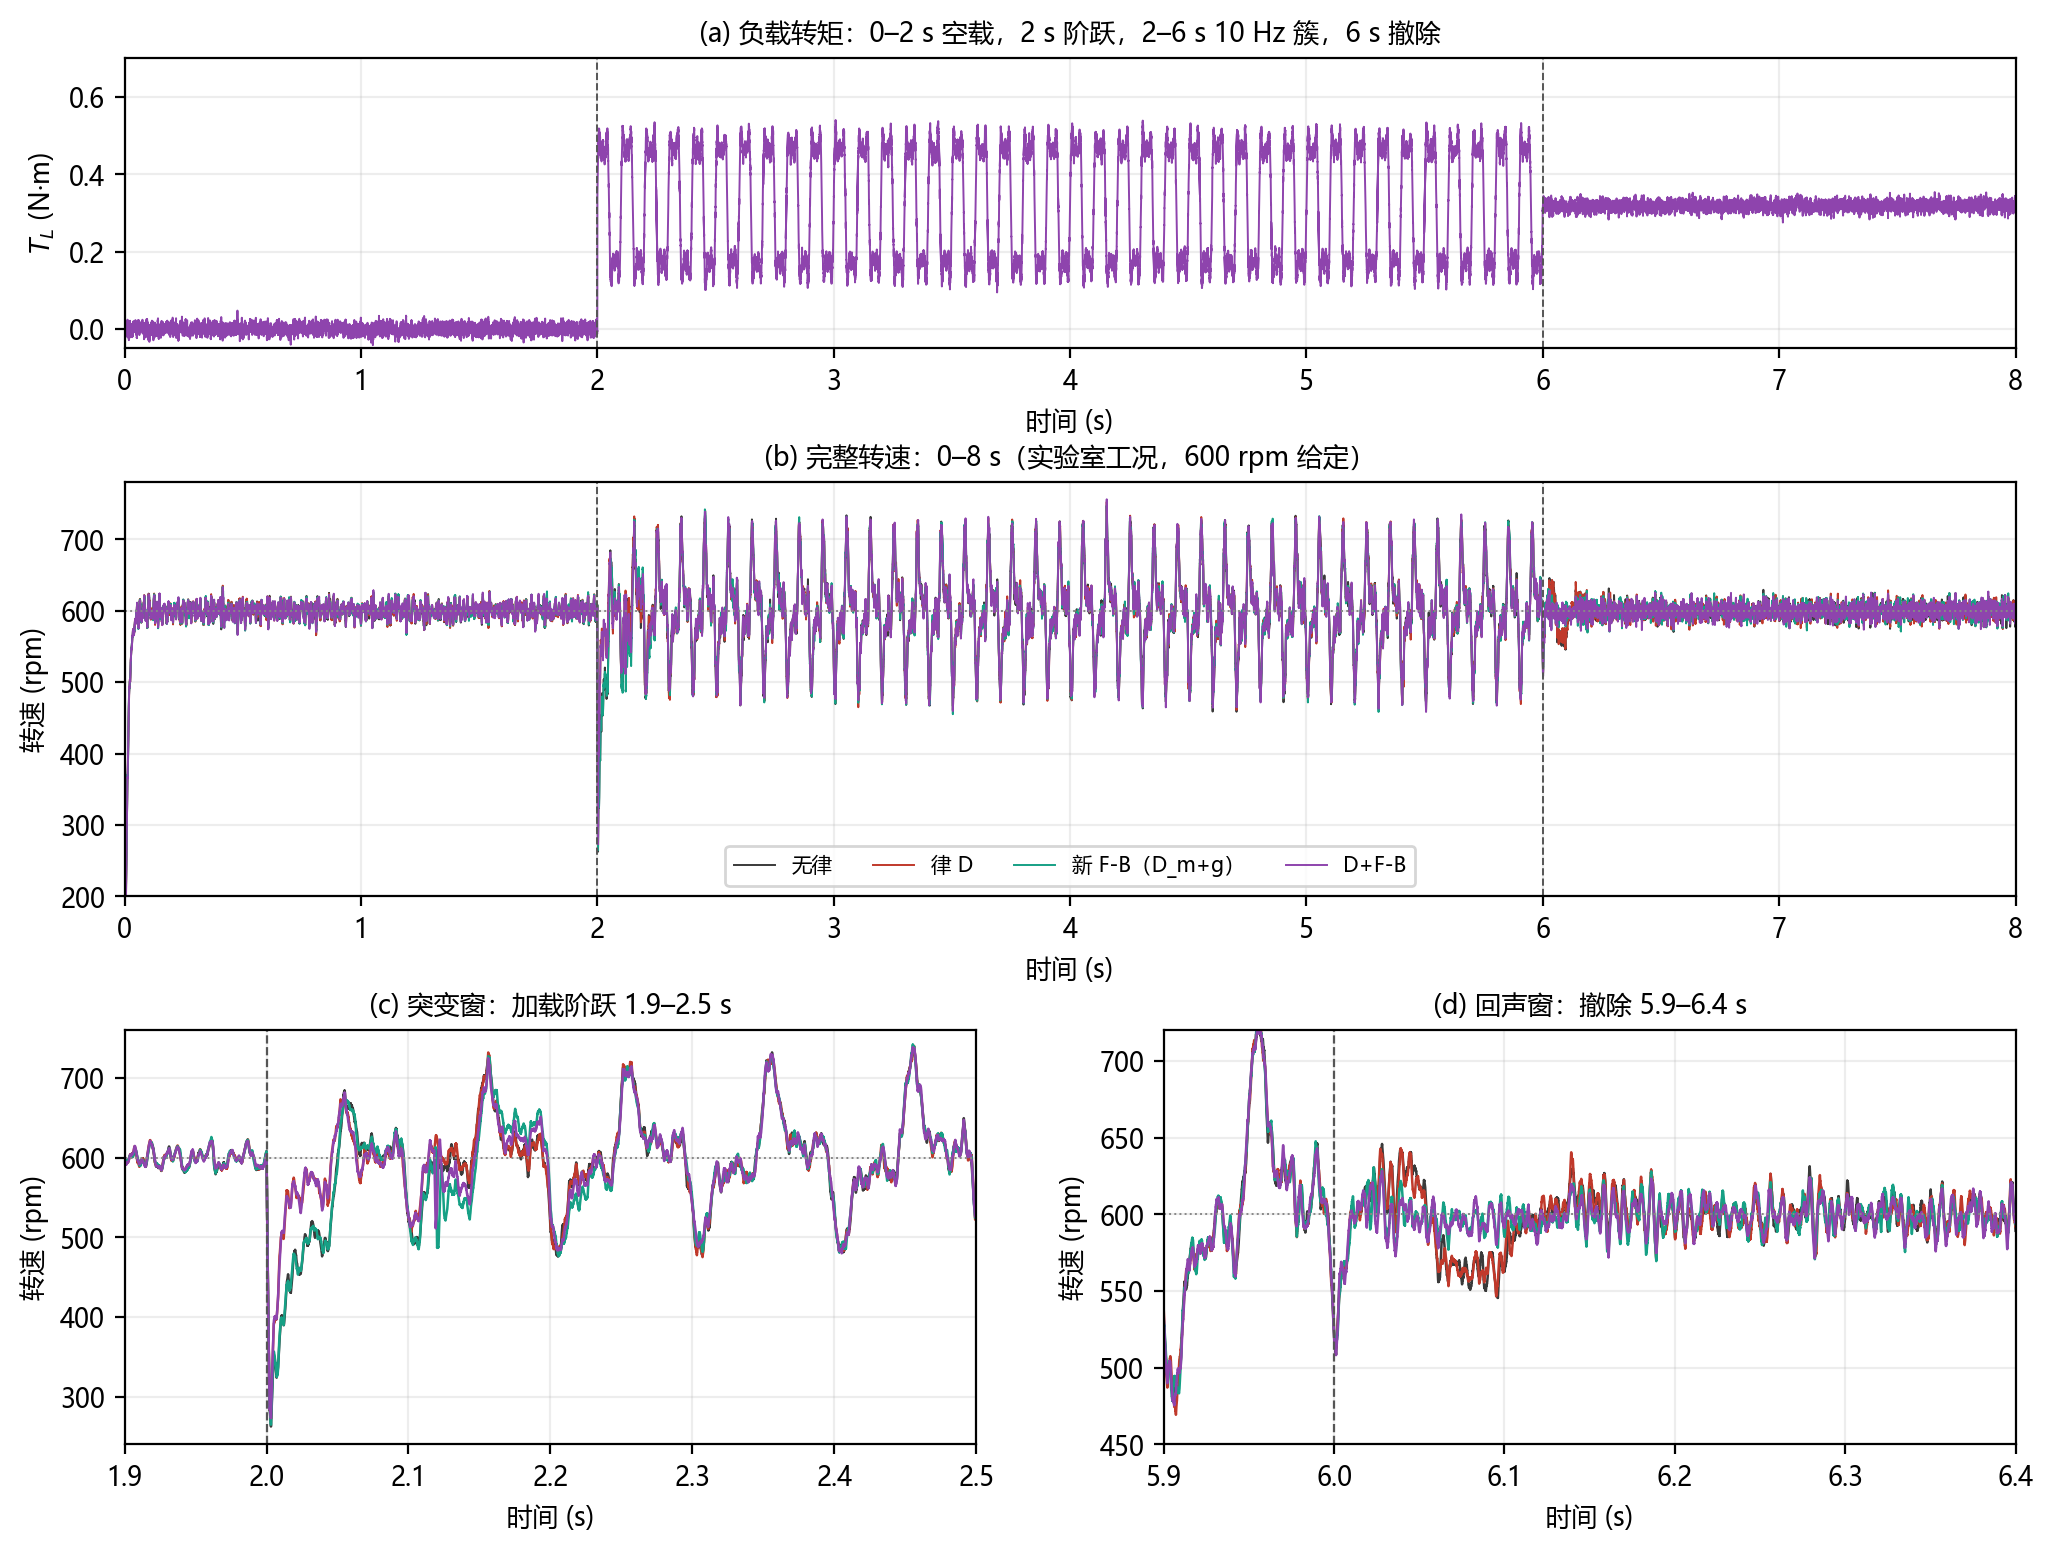
\includegraphics[width=0.99\textwidth]{fig_inv_speed_lab.png}
\caption{\textbf{实验室工况：负载与完整转速}（$3$\,rpm / $0.1$\,A / $0.01$\,N$\cdot$m）：
(a) 负载转矩；(b) 完整转速 $0$--$8$\,s；(c) 突变窗 $1.9$--$2.5$\,s；(d) 回声窗 $5.9$--$6.4$\,s。转速为绝对转速。}
\label{fig:inv-speed-lab}
\end{figure}

\subsection{额定转速 600/900/1200 rpm（10/15/20 Hz）}\label{sec:speedcases}
实验室噪声、$8$ 种子；同时改额定转速 $n_{\rm ref}$ 与重复周期 $T=1/f$（不能只改负载频率）。

\begin{center}\footnotesize
\begin{tabular}{@{}lccc@{}}
\toprule
配置 & 600 rpm（10 Hz） & 900 rpm（15 Hz） & 1200 rpm（20 Hz）\\
\midrule
Base & $37.49$ / $-336.2$ & $33.09$ / $-340.1$ & $28.19$ / $-354.8$\\
律 D & $35.38$ / $-327.8$ & $32.11$ / $-334.4$ & $27.81$ / $-349.8$\\
F-B & $\mathbf{6.44}$ / $-342.2$ & $\mathbf{7.71}$ / $-343.9$ & $\mathbf{7.54}$ / $-355.2$\\
D$+$F-B & $\mathbf{4.94}$ / $-346.7$ & $\mathbf{7.06}$ / $-332.9$ & $\mathbf{6.89}$ / $-348.8$\\
\bottomrule
\end{tabular}
\end{center}
\noindent 单元格为“首周期 $10$\,Hz / 加载跌落”。读数：无律的回声随转速升高由 $37.5$ 降到 $28.2$
（高频被惯量衰减）；律 D 的相对收益由 $-5.6\%$ 缩到 $-1.3\%$、跌落由 $-2.5\%$ 缩到 $-1.4\%$；
F-B 的绝对回声保持在 $6.4$--$7.7$，相对收益 $82.8\%\to76.7\%\to73.3\%$（分母变小）；
D$+$F-B 在三个转速都最低。F-B 的跌落离散在 $600$\,rpm 最大（$\pm19.0$，种子 023 $-388.8$），
$900/1200$\,rpm 降到 $\pm4.6/\pm2.9$，均值接近 Base。

\begin{figure}[htbp]\centering
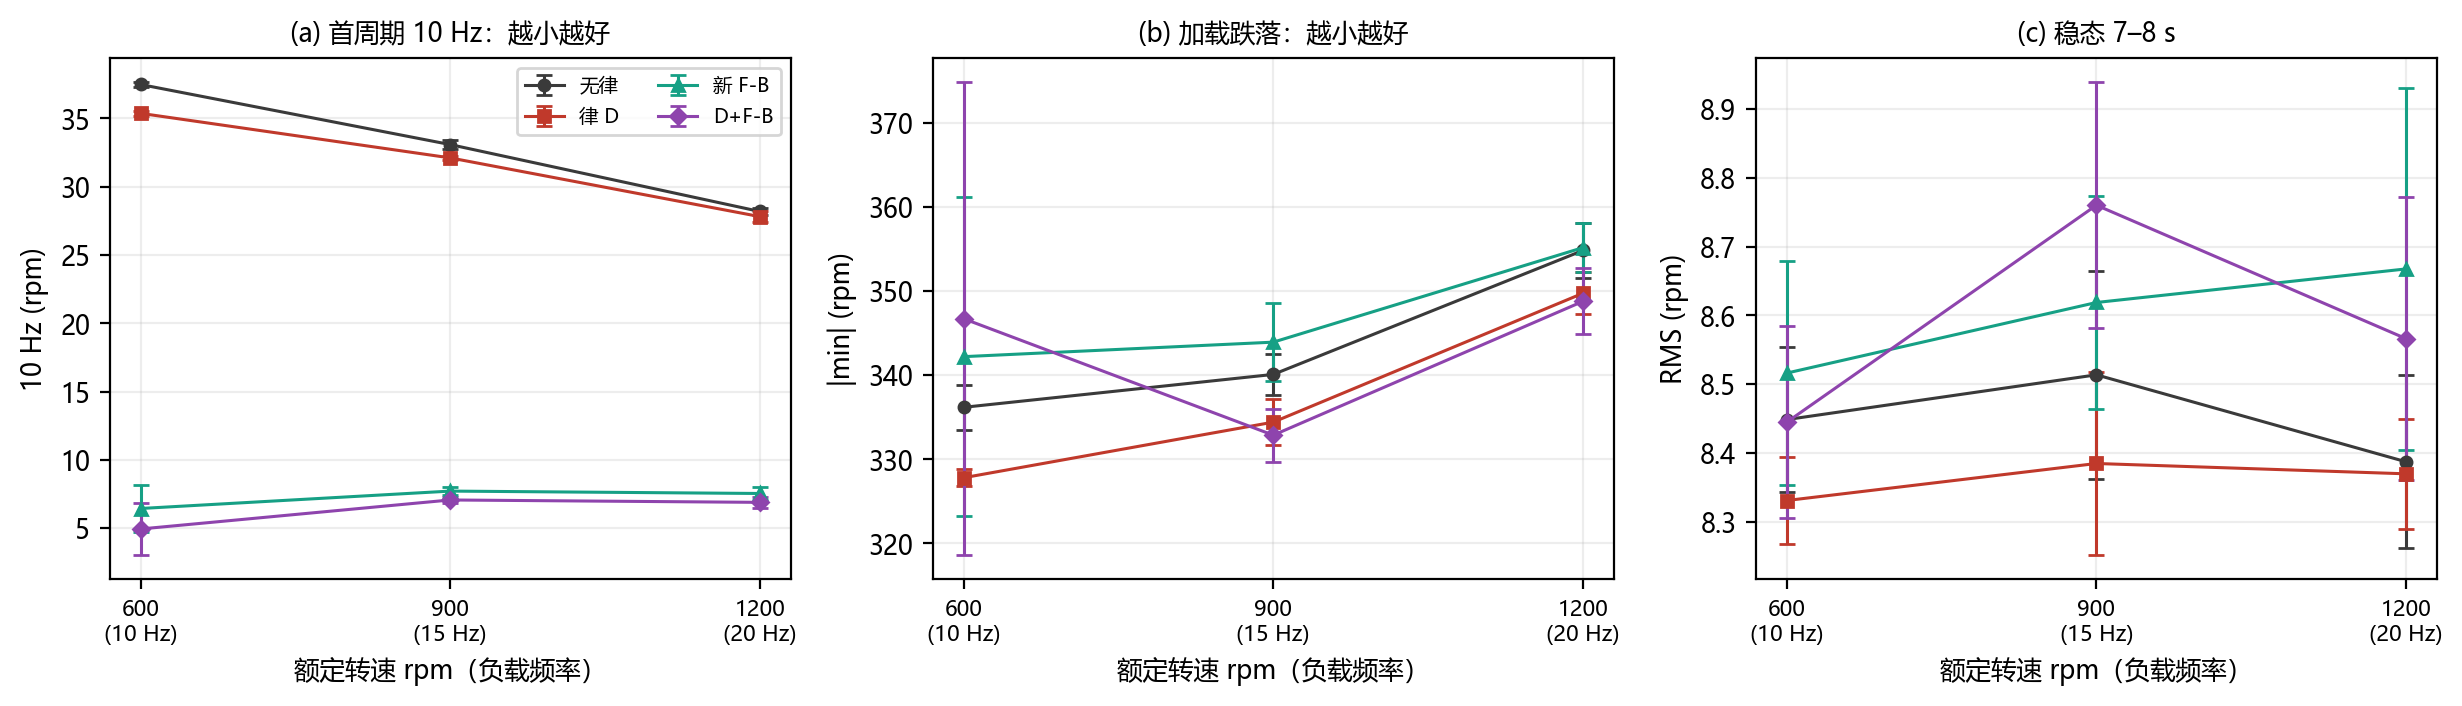
\includegraphics[width=0.99\textwidth]{fig_inv_speeds.png}
\caption{\textbf{三个额定转速/负载频率}（实验室噪声，8 种子）：(a) 首周期 $10$\,Hz；
(b) 加载跌落；(c) 稳态。F-B 的回声在三个转速都低，但 $600$\,rpm 的跌落误差棒明显更大。}
\label{fig:inv-speeds}
\end{figure}


\subsection{F-A 与 F-B：立即复位不是上界}
\begin{center}\footnotesize
\begin{tabular}{@{}lccc@{}}
\toprule
配置 & 首周期 $10$\,Hz & 加载跌落 & 稳态\\
\midrule
Base & $39.05\pm0.47$ & $-337.23\pm3.83$ & $18.77$\\
F-B（立即触发） & $6.20\pm2.65$ & $-337.17\pm4.64$ & $18.76$\\
F-A（$\tau=0$，立即） & $19.14\pm0.78$ & $-337.23\pm3.83$ & $18.59$\\
F-A（$\tau=20$\,ms） & $\mathbf{2.73\pm0.94}$ & $-337.23\pm3.83$ & $18.76$\\
\bottomrule
\end{tabular}
\end{center}
“立即复位”的 F-A 反而比 F-B 差；延后 $20$\,ms 的 oracle 最好。复位时刻扫描（种子 018/021）
在 $20$--$25$\,ms 取最小（$1.8$--$4.4$），$40$\,ms 回到 $23$\,rpm——旧时序律 $A_0(\tau)$ 的
单调性在真实对象上不成立。原因是复位注入 $-v$，相位不对时与首周期回声相加；F-B 的
$11$--$20$\,ms 检测滞后恰好落在最优附近，因此胜过“立即复位”的 F-A（图~\ref{fig:inv-fa}）。
注意：这里的“回声”按\emph{首周期 10 Hz} 定义；若改看 $6.0$--$6.1$\,s 的峰值，F-A 立即为 $129.9$、律 D 为 $105.2$（种子 018）——F-A 立即降低了 10 Hz 残余，但复位尖峰更大；两个指标不可互相替代。

\begin{figure}[htbp]\centering
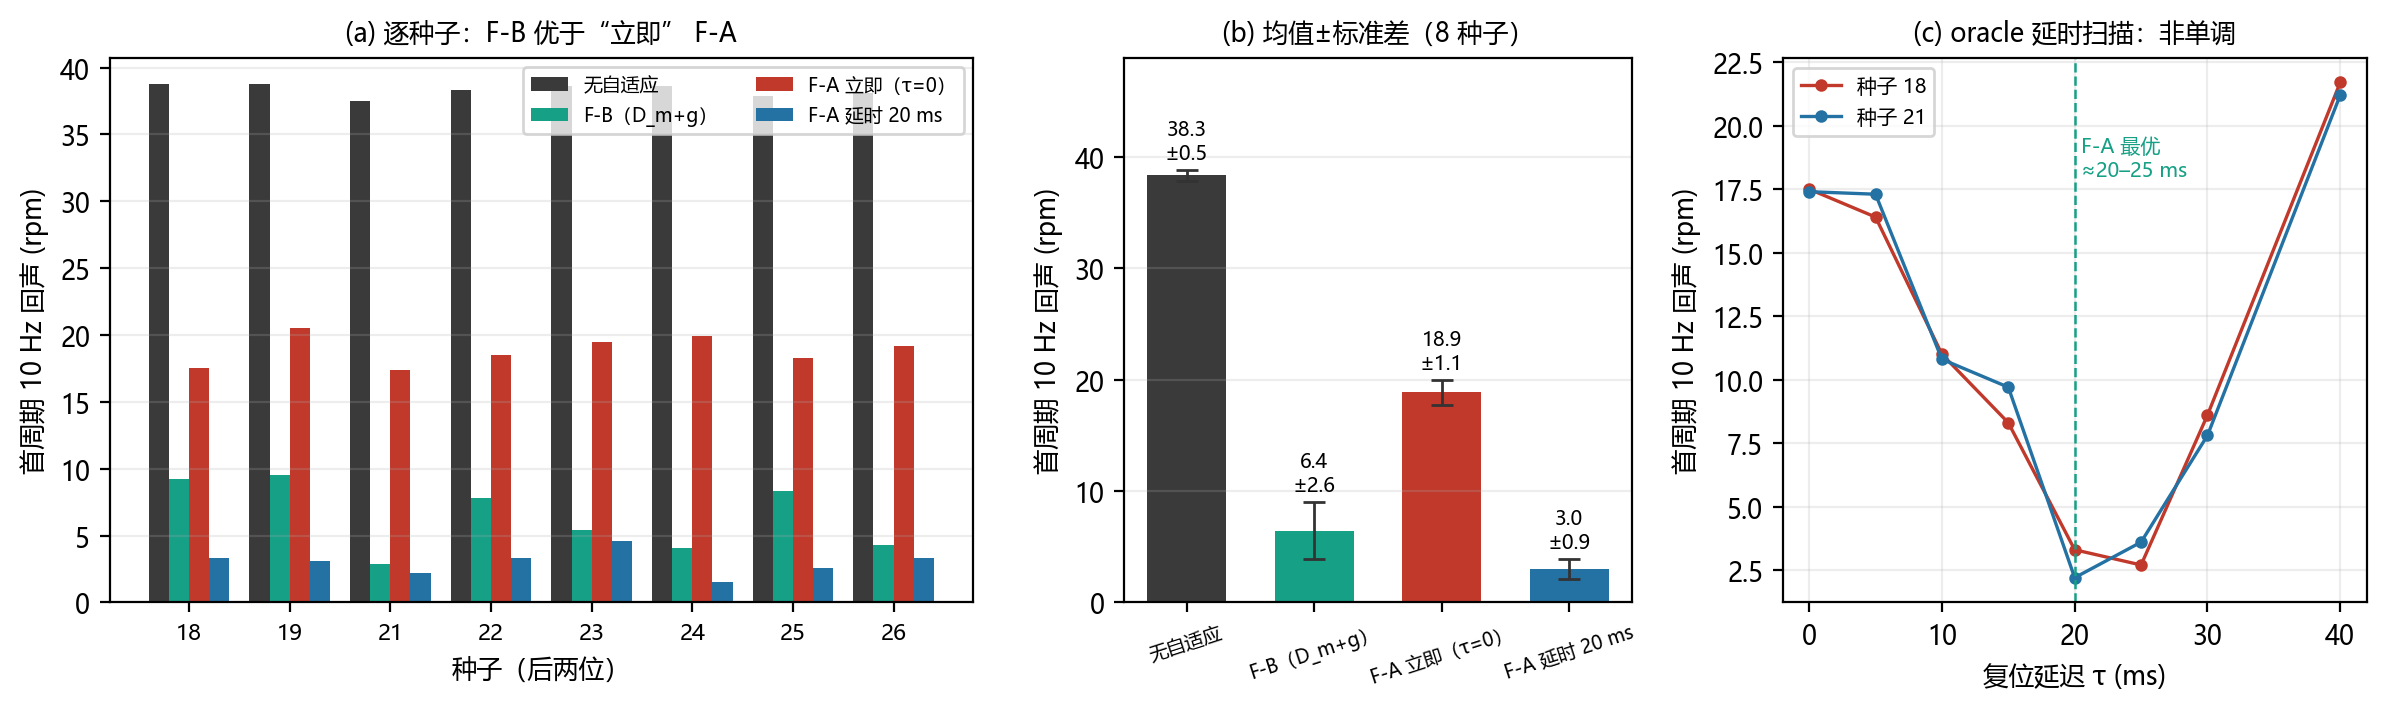
\includegraphics[width=0.99\textwidth]{fig_inv_fa.png}
\caption{\textbf{F-B 与 F-A 对比}。(a) 逐种子：F-B 优于“立即”F-A；(b) 均值$\pm$标准差；
(c) 复位时刻扫描：最小值在 $20$--$25$\,ms，非单调。}
\label{fig:inv-fa}
\end{figure}

\subsection{本节适用边界（如实披露）}
\begin{enumerate}
\item[(P1)] \textbf{死区是平均电压误差模型}，不是逐开关“上下管全关 + 二极管续流”的状态机；
      未建模二极管反向恢复、开关损耗、母线电容/LC 与磁饱和。
\item[(P2)] \textbf{离散化}：$2\,\mu$s 步长、$1$\,ms 速度环、$10$\,kHz 采样；
      $E_v$ 的 $T$ 窗按 $1$\,ms 离散实现，积分误差 $O(1/N)$；开关纹波对 $D_m$ 只由仿真量化。
\item[(P3)] \textbf{噪声口径}：dq 采样噪声按 $\pm0.2$\,A 均匀注入，转速 $6$\,rpm（$1\%$）、负载 $0.025$\,N$\cdot$m；
      若改逐相注入，dq 等效噪声不同。
\item[(P4)] \textbf{反相事件}：清空型 F-B 不适用（$8/8$ 种子 $0$ 触发、退化为基线
      $174.0\pm0.9$\,rpm），需 $\alpha=-1$ 的方向判别；本节的“F-B”只针对撤除。
\item[(P5)] \textbf{台架}：$D_m>0.2$、$g<0.05$ 的工程余量需在真实驱动器上复测；
      本节是仿真，不是实测。
\end{enumerate}

\section{适用范围之外（如实披露）}\label{sec:limit}
\subsection{律 F 的检测量与门控（真实对象）}\label{sec:fb-dilemma}
本版 F-B 不再用 $e_1$ 快/慢包络比值，而用记忆失配
\begin{equation}
D_m(t)=\frac{\bigl|E_v(t)-E_v(t-T)\bigr|}{E_v(t-T)+\varepsilon_v},
\qquad E_v(t)=\frac1T\int_{t-T}^{t}v^2\,\mathrm d\tau ,
\label{eq:Dm-report}
\end{equation}
触发条件为 $D_m>0.2$、$g<0.05$（$g$ 为 $e_1$ 的 $T$ 窗均值检测器，挡加载阶跃）、冷却 $0.3$\,s。
真实对象 $8$ 种子：首周期 $10$\,Hz 由 $39.05$ 降到 $6.20$（$-84.1\%$），与律 D 组合
$5.69$（$-85.4\%$）；跌落/稳态/电流不劣化；加载段 $0$ 次误触发；首触发 $6.011$--$6.02$\,s。
旧包络比值在同一对象上 $k=1.8$ 零触发（事件 $R=1.32$，与加载段 $1.3\sim1.5$ 重叠），
$k=1.3$ 虽在 $6.004$\,s 命中，但跌落 $-334\to-380$、加载段 $7$ 次误触发，已否决。

F-A 是“复位时刻/相位已知”的 oracle，不是触发律；但\textbf{立即复位（$\tau=0$）不是上界}：
实测 $\tau=0$ 为 $19.14$、$\tau=20$\,ms 为 $2.73$、F-B 为 $6.20$；复位时刻扫描最小值在
$20$--$25$\,ms，$40$\,ms 回到 $21$\,rpm。原因是复位注入 $-v$，相位不对时与首周期回声相加；
旧时序律 $A_0(\tau)$ 的单调性在真实对象上不成立。反相事件需 $\alpha=-1$ 的方向判别，
清空型 F-B 在反相下 $8/8$ 种子 $0$ 触发（退化为基线 $174.0\pm0.9$\,rpm），不可复用。

\subsection{其他边界}
\begin{enumerate}
\item[(F1)] \textbf{参数口径不可互引}：真实对象的数必须同时写明 $f_{ci}$、$\beta_3$、$\tau_0$、
      $D_m$ 阈值、$g_{\max}$、PWM/死区与噪声口径；旧一阶对象的数（如 $66.80\to48.36$、
      F-B $51.7$）不得与本节的数混引。
\item[(F2)] \textbf{$D_m$ 的界}：确定性上界 $D_m\le1+\bar v^2/\varepsilon_v$；$0.2$ 的工程余量
      由实测标定，随机噪声下的误报/漏报率未给解析界。
\item[(F3)] \textbf{F-A 的口径}：立即复位不是上界，上界应取 $\inf_\tau A_0(\tau)$；
      固定延时、裸 $v$ 阈值、$20$\,ms 正交相位三条相位等待路线均为负结果
      （固定延时、裸 $v$ 阈值、$20$\,ms 正交相位均未通过），需更低延迟的相位估计或前馈。
\item[(F4)] \textbf{证明的边界}：复位 UUB 与 Zeno 与检测器无关（只依赖冷却与有益跳变），
      但随机噪声、PWM/死区离散化不在确定性证明内；开关级对象的稳定性只由仿真给出。
\item[(F5)] \textbf{其他未做项}：死区逐开关状态机、母线电容/LC、磁饱和、台架实测；
      反相 $\alpha=-1$ 的方向判别（MMAE）未证明、未接入。
\end{enumerate}

\section{符号与参数表（答辩自查）}\label{sec:sym}
本表只列\textbf{真实逆变器对象}（\texttt{pmsm\_inv\_sim}）的定稿参数；旧一阶/降阶电流环对象的
参数与数字已从正文删除。加粗者为易被追问、正文中易漏标的参数。

\begin{center}\footnotesize
\setlength{\tabcolsep}{3pt}
\begin{tabular}{@{}llll@{}}
\toprule
类别 & 参数 & 符号 & 取值\\
\midrule
电机 & 相电阻 / 相电感 & $R$ / $L_d=L_q$ & $0.175\,\Omega$ / $0.57$\,mH\\
 & 磁链 / 极对数 & $\psi_f$ / $p$ & $0.01683$\,Wb / $4$\\
 & 转动惯量 & $J$ & $1.89\times10^{-5}$ kg$\cdot$m$^2$\\
 & 额定转矩 / 电流 & $T_{\rm rated}$ / $I_{\rm rated}$ & $0.637$ N$\cdot$m / $6.5$\,A（驱动器 $21$\,A）\\
\midrule
逆变器 & 母线 / 开关频率 & $V_{dc}$ / $f_{sw}$ & $60$\,V / $10$\,kHz\\
 & 死区 / 器件压降 & $T_d$ / $V_d$ & $2\,\mu$s / $0.9$\,V\\
 & 导通电阻 & $R_{on}$ & $10$\,m$\Omega$\\
\midrule
电流环 & 闭环带宽 & $f_{ci}$ & $2$\,kHz\\
 & PI 增益 & $k_p^i$ / $k_i^i$ & $7.16$ V/A / $2.20\times10^{3}$ V/(A$\cdot$s)\\
\midrule
速度环 & 比例增益 / 观测器带宽 & $k_p$ / $\omega_o$ & $75.36$ / $500$ rad/s\\
\midrule
重复通道 & 周期 / 内模增益 & $T$ / $\beta_3$ & $0.1$\,s / $4000$\\
 & 低通常数 / 遗忘因子 & $\tau_0$ / $Q_0$ & $20$\,ms / $0.98$\\
 & 饱和系数 & $\zeta$ & $0.2$\\
\midrule
律 F-B & 失配阈值 / 归一化下限 & $D_m$ / $\varepsilon_v$ & $0.2$ / $1\times10^{-6}$\\
 & 门控阈值 / 冷却 & $g_{\max}$ / $T_c$ & $0.05$ / $0.3$\,s\\
\midrule
噪声 & dq 采样噪声 & --- & $\pm0.2$\,A（均匀，$10$\,kHz）\\
 & 转速 / 负载噪声 & --- & $6$\,rpm（$1\%$）/ $0.025$\,N$\cdot$m（标准；三档见 \S\ref{sec:pmsm}）\\
\midrule
时序 & 积分 / PWM / 速度环 & $\Delta t$ / $T_{pwm}$ / $T_s$ & $2\,\mu$s / $100\,\mu$s / $1$\,ms\\
 & 编码器 & --- & $2500$ PPR（$4\times$）\\
\midrule
工况 & 阶跃 / 不对中簇 & --- & $0.50$ 额定 / $10$\,Hz、$A=0.30$（$2$--$6$\,s）\\
\bottomrule
\end{tabular}
\end{center}
\noindent\textbf{七窗口定义}：空载 $[0.5,2.0)$、加载瞬态 $[2.0,2.5)$、事件1 $[2.5,2.6)$、
事件2 $[3.0,3.5)$、事件后 $[3.5,4.0)$、持续段 $[4.0,6.0)$、稳态段 $[7.0,8.0)$ 秒。

\section{结论}\label{sec:concl}
% =====================================================================
\begin{enumerate}
  \item \textbf{建模}：一阶对象 $+$ 低通重复通道（内模）$+$ 灰箱 ESO $+$ 双通道自适应；三条回路共用驱动 $\ef=\tau\dot v$，故必须整体处理。
  \item \textbf{自适应律与实现逐条对应}（\S\ref{sec:law}）：驱动取\emph{零均值实参} $w=\phi\big((\ef^{2}-E_o)/(E_o+\varepsilon),c\big)$ 的\emph{快慢两路带通} $D=w_f-w_l$（$\tau_f^w=5T$、$\tau_l^w=50T$）；$Q$ 取\emph{单向死区} $\max(0,D)$。
  \item \textbf{一致有界性（UUB）}（§\ref{sec:uub}、注 \ref{rem:robust}）：$v$ 通道自持 UUB（界 $\beta_3/(1-Q_0)$，与 $e_1$ 无关）；ESO 误差界 $\frac{2\sqrt3}{\omega_o}\sqrt{\bar v^2+(H/\omega_o)^2}$；跟踪误差界 $\frac{b_0}{bk_p}(\sup|d|+\frac{b}{b_0}(\sup|x_2|+\bar v))$。\textbf{调度不放大界}：$g\in[0,1)$ 且 $\kappa\ge0$ $\Rightarrow$ 增益只增不减 $\Rightarrow$ 名义界即调度闭环的界；\textbf{仍开放}的是随机噪声下的界（不在确定性框架内）与界的收紧。
  \item \textbf{归一化与零均值实参的作用}（注 \ref{rem:zero-mean}）：零均值实参使 $\overline{D}\to0$，$Q$ 的平衡点回到 $1$ 附近、具备调节能力；恒正实参会把 $Q$ 单向压到底。
  \item \textbf{如实报告的边界}：见 \S\ref{sec:limit}（参数口径不可互引、$D_m$ 的噪声界、
        F-A 的立即复位不是上界、UUB 与检测器无关、台架待测）。
  \item \textbf{真实逆变器对象上的验证}（\S\ref{sec:pmsm}）：对象为三相 $10$\,kHz PWM、死区、
        反电动势、编码器量化与 $\pm0.2$\,A dq 采样。重整定 $\tau_0=20$\,ms、$\beta_3=4000$、
        $f_{ci}=2$\,kHz 后：(a) 律 D 仍是 Pareto 但收益缩小——跌落 $-337.23\to-331.39$\,rpm
        （$-1.7\%$）、回声 $39.05\to36.36$（$-6.9\%$）；(b) F-B 用记忆失配 $D_m+g$：
        首周期 $10$\,Hz $39.05\to6.20$（$-84.1\%$），与律 D 组合 $5.69$（$-85.4\%$），
        加载段 $0$ 误触发、跌落/稳态/电流不劣化；(c) 旧包络比值与旧一阶对象数字
        （$66.80\to48.36$、F-B $51.7$）已删除，不得再引用。
  \item \textbf{律 F 的检测量与相位}（\S\ref{sec:fb-dilemma}）：$D_m>0.2$ 且 $g<0.05$，
        首触发 $6.011$--$6.02$\,s；F-A 立即复位不是上界（$19.14$ 对延时 $20$\,ms 的 $2.73$），
        F-B 的 $11$--$20$\,ms 滞后恰好接近最优；固定延时、裸 $v$ 阈值、$20$\,ms 正交相位三种
        相位等待均为负结果；反相需 $\alpha=-1$，不得复用清空型 F-B。
\end{enumerate}


\section{接手说明（给下一个 agent）}\label{sec:handoff}
\noindent\textbf{现状}：本文档 v4.0 的\textbf{数值口径严格为真实逆变器对象}
（\texttt{pmsm\_inv\_sim}：三相 PWM、死区、反电动势、编码器量化、$\pm0.2$\,A dq 采样）；
旧一阶/降阶电流环对象的数字（$66.80\to48.36$、F-B $51.7$ 等）已从正文删除。
理论/证明部分（\S\ref{sec:model}--\S\ref{sec:verify}）仍在标幺一阶模型上给出，只用于结构性质。

\begin{center}\footnotesize
\begin{tabular}{@{}p{5.2cm}p{9.6cm}@{}}
\toprule
文件 & 职责\\
\midrule
\texttt{rcso\_v3.tex / .pdf / .html} & 本文档。\textbf{tex 是唯一源}；html 由 \texttt{python \_mkhtml.py rcso\_v3.tex} 生成\\
\texttt{proof\_lawD\_lawF.tex / .pdf} & 律 D / 律 F 的证明；F-B 为记忆失配 $D_m+g$，含 F-A 对比\\
\texttt{pmsm\_inv\_sim.py} & \textbf{唯一正式对象}：三相 PWM 逆变器 + PMSM + 采样\\
\texttt{fb\_cfg.py} & 律 F-B 配置入口（历史 \texttt{FB\_NEW/FB\_OLD}；真实对象用 \texttt{ff\_mism}）\\
\texttt{run\_inv\_lawd.py} & 律 D 的 8 种子（真实对象）\\
\texttt{run\_inv\_mism\_g.py} & 记忆失配 F-B 的 8 种子\\
\texttt{run\_inv\_fa.py / run\_inv\_fa\_delay.py} & F-A oracle 与复位时刻扫描\\
\texttt{plot\_inv\_*.py} & 出图（只读 JSON/npz）\\
\texttt{noise\_cfg.py} & 噪声单一入口（\texttt{i\_noise\_peak=0.3}）\\
\texttt{adrc\_eso\_closed.py} & 一阶核参照（非正式对象；仅回归/理论对照）\\
\texttt{pmsm\_dq\_sim.py} & 旧 dq 降阶对象（历史，不得用于新结果）\\
\bottomrule
\end{tabular}
\end{center}

\noindent\textbf{标准工作流}：
\begin{enumerate}
  \item \textbf{定口径}：真实对象参数（$f_{sw}=10$\,kHz、死区 $2\,\mu$s、$f_{ci}=2$\,kHz、
        $\beta_3=4000$、$\tau_0=20$\,ms、$D_m=0.2$、$g_{\max}=0.05$）；
        旧对象参数不得混入。
  \item \textbf{跑仿真}：正式数据一律用 \texttt{sim\_inv}（\texttt{pmsm\_inv\_sim}）；
        \texttt{adrc\_sim}/\texttt{sim\_mr3} 只作理论/回归对照。
  \item \textbf{存轨迹}：\texttt{np.savez} 保存 $t/y/i_q/i_d/i_a$，文件名带配置与日期。
  \item \textbf{出图}：脚本只读数据、不重新仿真；图注写清口径（步长、窗长、种子、噪声）。
  \item \textbf{改文本}：先改 \texttt{tex}；被替换的旧口径必须删除（文首版本纪律）。
  \item \textbf{重编}：本文档与附注 \texttt{xelatex} 两遍；HTML 用 \texttt{\_mkhtml.py} 生成并跑自检。
\end{enumerate}

\noindent\textbf{噪声口径（真实对象）}：三档工况（实验室/标准/恶劣）见 \S\ref{sec:pmsm}；
默认标准档：dq 采样噪声 \texttt{i\_noise\_peak}$=0.2$\,A（均匀 $\pm0.2$）、
转速 \texttt{sig\_n\_rpm}$=6$（$1\%$）、负载 \texttt{sig\_T\_nm}$=0.025$\,N$\cdot$m；旧的 \texttt{sig\_i\_A}$=0.2$ 只用于
\texttt{pmsm\_dq\_sim} 历史复现，不得写入真实对象结果。

\noindent\textbf{硬约束（违反即返工）}：
\begin{itemize}
  \item \textbf{对象铁律}：新数值只能来自 \texttt{pmsm\_inv\_sim}；旧一阶/降阶对象的结果不得引用。
  \item \textbf{版本纪律}：新旧口径不得并存；换对象必须同步删旧数。
  \item 律 F 定稿：$D_m>0.2$、$g<0.05$、冷却 $0.3$\,s；旧包络比值已否决。
  \item F-A 是 oracle，但\textbf{立即复位不是上界}：真实对象最优在 $20$--$25$\,ms；
        固定延时/裸 $v$/20\,ms 正交相位三种相位等待均为负结果。
  \item 反相事件需 $\alpha=-1$ 的方向判别，不得复用清空型 F-B。
  \item 出图只输出 PNG；\texttt{includegraphics} 指向 PNG。
\end{itemize}

\noindent\textbf{当前未完成}：论文台架数据仍是【待补】/[TO BE FILLED]；论文律 F 段需改用本文
$D_m+g$ 口径；死区逐开关状态机/母线 LC、反相 $\alpha=-1$、台架实测未做。

\noindent\textbf{交付前自检}：\texttt{xelatex} 0 error；HTML 自检通过、内嵌图齐全；
表内数字可由 JSON/npz 复算；正文不存在旧对象数字；新增结果标注真实对象参数。

\end{document}
